\documentclass[a4paper,11pt]{article}
\usepackage{jcappub}
\usepackage{txfonts}
\usepackage{threeparttable}
\usepackage{aas_macros}
\usepackage{graphicx}
\usepackage{subfigure}
\usepackage{url}
\usepackage{amsmath}


\title{Precision cosmology with time delay lenses: high resolution imaging requirements}
%\title{Cosmology with time delay lenses. High resolution imaging requirements}
\author[1]{Xiao-Lei Meng,}
\author[1,2]{Tommaso Treu,}
\author[1,2]{Adriano Agnello,}
\author[3]{Matthew W.~Auger,}
\author[1,2]{Kai Liao,}
\author[4]{Philip J. Marshall}

\affiliation[1]{Department of Physics, University of California, Santa Barbara, CA 93106, USA}
\affiliation[2]{Physics and Astronomy Building, 430 Portola Plaza, Box 951547, Los Angeles, CA 90095-1547, USA}
\affiliation[3]{Institute of Astronomy, University of Cambridge, Madingley Road, Cambridge CB3 0HA, UK}
\affiliation[4]{Kavli Institute for Particle Astrophysics and Cosmology, Stanford University, 452 Lomita Mall, Stanford, CA 94305, USA}

\emailAdd{xlmeng919@gmail.com}

\date{Accepted . Received }

\abstract{
Lens time delays are a powerful probe of cosmology, provided that the
gravitational potential of the main deflector can be modeled with
sufficient precision. Recent work has shown that this can be achieved
by detailed modeling of the host galaxies of lensed quasars. The
distortion of the images as measured over large number of pixels
provides tight constraints on the difference between the gravitational
potential between the quasar image positions, and thus on cosmology in
combination with the measured time delay. We carry out a systematic
exploration of the high resolution imaging required to eploit the
thousands of lensed quasars that will be discovered by current and
upcoming surveys with the next decade. Specifically we simulate
realistic lens systems as imaged by the Hubble Space Telescope (HST),
James Webb Space Telescope (JWST), ground based adaptive optics images
taken with Keck or the Thirty Meter Telescope (TMT). We compare the
performance of these pointed observations with that of images taken by
the Euclid-VIS, Wide-Field Infrared Survey Telescope (WFIRST) and
Large Synoptic Survey Telescope (LSST) surveys. We use as our metric
the precision with which the slope $\gamma'$ of the total mass density
profile $\rho_{tot}\propto r^{-\gamma'}$ for the main deflector can be
measured. Ideally, we require that the statistical error on $\gamma'$
be less than 0.02, thus being subdominant with respect to other
sources of random and systematic uncertainties. We find that survey
data will likely have sufficient depth and resolution to meet the
target only for the brighter gravitational lens systems, comparable to
those discovered by the SDSS survey. For fainter systems, that will be
discovered by current and future surveys, targeted follow-up will be
required. However, the exposure time per target will be of order a few
minutes per system with upcoming facilitites, such as JWST, the Keck
Next Generation Adaptive Optics System, and TMT, thus making the
follow-up of hundreds of systems a pratical and efficient cosmological
probe.}

\keywords{}

\begin{document}
\newcommand\farcs{\hbox{$.\!\!^{\prime\prime}$}}
\maketitle
\flushbottom


\section{Introduction}
%\textbf{[TT to put introfirst here; introduce `informative pixels' that will be referred to in Sect.s 2 and 3; mention that we're basically observing how radial magnification changes across the lens, so that we need to understand how that is affected by PSF, pixel-size, and S/N ratio.]}

In the past few years, gravitational time delays (Refsdal 1964 \citep{1964MNRAS.128..307R})
have emerged as a powerful and cost effective cosmological
probe. Studies based on blind analysis have shown that a single system
consisting of multiple images of a background quasar (at redshift
$z_s$) lensed by a foreground massive elliptical galaxy at redshift
$z_d$ can be used to measure the so-called time delay distance with an
uncertainty of 6-7\% (Suyu et al. 2010 \citep{2010ApJ...711..201S}, 2013 \citep{2013ApJ...766...70S}, 2014 \citep{2014ApJ...788L..35S}). The time
delay distance $D_{\Delta t}$ gives a direct measurement of the Hubble
constant and allows one to break some the main degeneracies in the
interpretation of cosmic microwave background data, thus providing
tight constraints on parameters such as curvature and dark energy
equation of state
(Coe \& Moustakas 2009 \citep{2009ApJ...706...45C}, Linder 2011 \citep{2011PhRvD..84l3529L}, Weinberg 2013 \citep{2013PhR...530...87W}, Suyu 2012 \citep{2012MNRAS.426..868S}, Suyu et al. 2014 \citep{2014ApJ...788L..35S}). The
time delay distance measurement of H$_0$ is comparable in terms of
information content to that obtained via the cosmic distance ladder
(Riess et al. 2011 \citep{2011ApJ...730..119R}, Freedman et al. 2012 \citep{2012ApJ...758...24F}), in that is based on absolute distances and completely
independent on the properties of the universe at $z>z_s$. Importantly,
time delay distances are independent of the local distance ladder and
thus provide a crucial test of any potential systematic
uncertainties. Furthermore, being independent, the cosmic distance
ladder and time delay distance constraints on H$_0$ can be
statistically combined for additional gains in precision.

From an observational point of view, the attainment of precise and
accurate time delay measurements relies on a few important
ingredients. First, monitoring of the lensed quasars is required to
obtain time delays with a few percent uncertainties. Dedicated
monitoring campaigns have shown that this precision is achievable with
1-2m class telescopes at present time (Tewes et al. 2013
\citep{2013A&A...556A..22T}), or in the radio (Fassnacht et al. 2002
\citep{2002ApJ...581..823F}). In the future, the exploitation of
larger samples of lenses will require monitoring campaigns on 2-4m
telescopes (Treu et al. 2013 \citep{2013arXiv1306.1272T}), or the
deployment of long term high-cadence monitoring surveys, like the LSST
(Liao et al. 2015 \citep{2015ApJ...800...11L}). Second, the
spectroscopic redshift of the source and deflector must be measured
. For current samples, this is typically a relatively straightforward
step, requiring short exposures on 4-10m class telescopes (Fassnacht
\& Cohen 1998 \citep{1998AJ....115..377F}, Eigenbrod et al. 2007
\citep{2007A&A...465...51E}).  Third, the gravitational potential of
the main deflector needs to be constrained by the data so that the
uncertainty on its difference between the location of the images is
also of order 3\%. This goal can be achieved by studying the extended
structure of the lensed quasar host galaxy, and the stellar kinematics
of the deflector galaxy (Treu \& Koopmans 2002
\citep{2002MNRAS.337L...6T}, Koopmans et al. 2003
\citep{2003ApJ...599...70K}, Suyu et al. 2010
\citep{2010ApJ...711..201S}, Suyu et al. 2013
\citep{2013ApJ...766...70S}, Suyu et al. 2014
\cite{2014ApJ...788L..35S}).  Fourth, the combined effects of the
inhomogenous mass distribution along the line of sight need to be
taken into account. Recent work has shown that the line of sight
effects can be sufficiently characterized by measuring the properties
of galaxies and weak lensing signal in the field of the main
deflector, and comparing with simulated lines of sight (Suyu et
al. 2010 \citep{2010ApJ...711..201S}, 2013
\citep{2013ApJ...766...70S}, 2014 \citep{2014ApJ...788L..35S}, Greene
et al. 2013 \citep{2013ApJ...768...39G}, Collett et al. 2013
\citep{2013MNRAS.432..679C}).

However, whereas current samples have been limited to a few lenses,
current and onging surveys (add references to DES, PANSTARRS, HSC,
ATLAS) will discover 100s of lenses. These large samples will be
extremely powerful cosmographic probes
(Coe \& Moustakas 2009 \citep{2009ApJ...706...45C}, Linder 2011 \citep{2011PhRvD..84l3529L}), provided that sufficient follow-up
data will be available (Treu et al. 2013 \citep{2013arXiv1306.1272T}). In this paper we carry out a
feasibility study for future time delay surveys, focusing on the
high-resolution imaging requirements. Specifically, we aim to
investigate whether sufficient information will be available from
survey data, or whether dedicated follow-up will be necessary. If
dedicated follow-up will be necessary, we aim to provide an estimate
of the amount of time that will be required per system. The
multi-pronged nature of time delay lens follow-up makes it natural to
follow the approach of addressing each component of the follow-up
independently. The monitoring and spectroscopic follow-up requirements
are described, e.g., by Eigenbrod et al. 2005 \cite{2005A&A...436...25E}, Linder 2015 \cite{2015PhRvD..91h3511L}.

In order to make the problem tractable and the results general, we
need a single simple metric to evaluate the quality of imaging
data. In short, we need to quantify our ability to measure how the
deflection angle (i.e. the derivative of the lensing potential) varies
between the images, and thus how the extended images of the quasar
host galaxy are stretched across the image. In practice, our ability
to constrain the differential magnification will depend on the
resolution of the data as well as on the number of pixels where the
source is detected (hereafter {\it informative pixels}).

We choose to adopt as our metric the slope $\gamma'$ of the total mass
density profile of the form $\rho_{\rm tot}\propto r^{-\gamma'}$ as
measured by fitting elliptical power law models to the data. This
profile is the simplest one that provides a realistic description of
galaxy scale lenses (Treu 2010 \citep{2010ARA&A..48...87T}), and the uncertainty $\gamma'$
has been shown to be approximately proportional to the uncertainty on
the gravitational potential differences and thus the time delay
distance
(Kochanek 2002 \citep{2002ApJ...578...25K}, Wucknitz 2002 \citep{2002MNRAS.332..951W}, Suyu 2012 \citep{2012MNRAS.426..868S}). 
Intuitively, $\gamma'$ is directly related to the variations of the
lensing potential. In fact, if $\gamma'=2$ (the so-called isothermal
profile) the deflection angle is constant across the image and
therefore all the images will appear to have the same radial
magnification. If the profile is steeper/shallower, radial
magnification will vary across the image, thus giving rise to images
of different widths.

Naturally, for a real measurement it is important to explore different
profiles and the role of the choice of the profile in the
uncertainties. However, our goal is to estimate minimal requirements
on the data quality. If the data quality is insufficient to constrain
$\gamma'$ it will also be insufficient to constrain more flexibile
models. Likewise, systematic errors not considered in this paper, such
as those arising from incomplete knowledge of the PSF, will only
increase the error budget. Thus, in order to leave room for additional
sources of uncertainty in the error budget, we set a rather stringent
requirement of 0.02 uncertainty of $\gamma'$ (corresponding
approximately to 2\% per system on time delay distance). In other
words, our target corresponds to the requirement that the {\it
statistical} error arising from the image quality be subdominant with
respect to those arising from modeling uncertainties, time delays, and
line of sight effects.

This paper is organized as follows. In Section 2, we summarize the
characteristics of the telescopes and instruments simulated as part of
this work. Then, in Section 3, we describe the properties of the
simulated lenses. Next, in Section 4 we describe the procedure used to
carry out the inference.  Our results are presented in Section
5. Finally, we discuss and summarize our work in Section 6. Throughout
this paper, all magnitudes are given in the AB system. Even though our
findings are independent of any cosmology, we adopt a spatially flat
$\Lambda$CDM cosmology with $\Omega_{\rm{m}} = 0.3$, $\Omega_{\Lambda}
= 0.7$, and the Hubble constant $H_{0} = 70~\rm km~s^{-1}~Mpc^{-1}$
when calculating distances.

\section{Summary of simulated instrumental setups}

We aim to carry out a systematic exploration of imaging requirements
given current and future facilities. For a given lens system, the
instrumental setup drives our ability to constrain $\gamma'$ in a
number of ways. First, the signal-to-noise ratio depends on the
exposure-time adopted, sky or background noise in a chosen band, and
the instrumental readout noise. Second, the pixel-size and the
point-spread function (PSF) properties determine how finely one can
map the system being observed, hence how robustly the deflections on
either side of the lens can be quantified.
 
Here we summarize the main properties of instruments that will be
considered in our simulations. In an effort to balance completeness
with feasibility, we consider a suite of instruments that include
ground and space based telescopes, and cadenced surveys where the
total exposure cannot be set arbitrarily. Some of the choices are
representative of a class of telescopes/instruments, for example we
expect the performance of Keck Adaptive Optics to be a useful guidance
for adaptive optics systems on other 8-10m class telescopes, and that
of the Thirty Meter Telescope to be a guidance for other planned
20-30m class telescopes.

Table~\ref{tab:telescopes parameters} and
figure~\ref{fig:zp_wavelength} display the main properties of the
telescopes that are needed when generating images of mock
gravitational lenses, taken from the instrument
websites. Figure~\ref{fig:PSF_montage} shows the typical PSF of each
instrument. In order to facilitate comparisons between instruments and
telescopes, whenever possible we selected the filter/band for each
configuration that is closer to the $I$-band in the optical and the
$K'$-band in the near infrared. A brief description of each setup
follows.

\begin{enumerate}

\item  The Advanced Camera for Surveys (ACS) is chosen as our reference optical imager on board the Hubble Space Telescope (HST). In the chosen F814W filter its performance is comparable to those of WFC3 (slightly higher sensitivity and coarser pixel size). For simplicity, we neglect charge transfer inefficiency effects, assuming that they are negligible or can be corrected to the desired level. The PSF is simulated using the Tiny Tim software (Krist 1993 \cite{1993ASPC...52..536K})
%Its properties are taken from Space
%    Telescope Science Institute and HST Exposure Time Calculator
%    website \footnote{\url{http://etc.stsci.edu}}.
    
\item The Near Infrared Camera (NIRCAM) on board the James Webb Space Telescope (JWST) is chosen as the next space based imaging capability. We select the broad F200W filter, where the image quality is virtually diffraction limited. 

% infrared-optimized space telescope which obtains four instruments:
% near-infrared camera, mid-infrared instrument, near-infrared
% multi-object spectrograph, and a tunable filter imager. Its
% scientific goals include exploring planetary systems, star evolution,
% galaxy-scale theme, and remote dark ages (Gardner et al. 2006
% \cite{2006SSRv..123..485G}). We determinate instrument properties by
% JWST Exposure Time Calculator
% \footnote{\url{http://jwstetc.stsci.edu}}. F200W band is selected to
% consider. The pixel size is $0.032^{\prime\prime}$/pixel. Zero point,
% readout noise, and background noise are calculated from count rates
% at fixed exposure time.

\item The current and planned adaptive optics systems (hereafter LGSAO \& NGAO; Wizinowich et al. \citep{2006PASP..118..297W}, \citep{2010SPIE.7736E..0KW}, respectively) at the W.M.Keck Observatory are chosen to represent current and upcoming AO performance on 8-10m class telescopes. We consider the current instrument NIRC2, although further gains might be possible with an instrument upgrade in conjuction with the AO system upgrade. We adopt the typical configuration used for studies of gravitational lens systems (Fassnacht \& Cohen 1998 \citep{1998AJ....115..377F}): $K'$ filter, MCDS readout mode, read number $N=16$, and narrow camera mode. A real observed PSF is used for the current AO system. The simulated PSF and performance characteristics of NGAO have been kindly provided by the NGAO team.
    
\item The infrared imager and spectrograph IRIS (Larkin et al. 2010 \citep{2010SPIE.7735E..29L}) working behind adaptive optics on the thirty Meter Telescope (TMT) is selected to represent the performance of the extremely large telescopes that will be operational in the next decade. IRIS is expected to be close to diffraction limited in the $K'$ band. The simulated PSF and performance characteristics of TMT-IRIS have been obtained from the IRIS team, from the TMT Exposure Time Calculator (ETC) \footnote{\url{http://tmt.mtk.nao.ac.jp/ETC_readme.html}} and from the paper by Do et al. (2014) \citep{2014AJ....147...93D}.
    
\item Euclid is a space survey telescope planned to be launched by the European Space Agency. Euclid has two instruments: a high-resolution visible imager, and a NIR imaging instrument.
%It aims to investigate the nature of dark energy, dark matter, and gravity by using cosmological probes, such as weak gravitational lensing and baryon acoustic oscillations (Laureijs et al. 2011). 
We study the performance of the high-resolution visible imager, the
more suitable to detailed gravitational lensing work, with the
standard survey parameters.  The instrument properties are taken from
Schweitzer et al. 2010
\cite{2010SPIE.7731E..1KS}, Penny et al. 2013
\cite{2013MNRAS.434....2P} and Cropper et al. 2014
\cite{2014SPIE.9143E..0JC}.
Since the PSF is proprietary to the Euclid team, we adopt for simplicity a Gaussian function with full width half maximum $0\farcs18$.
%The readout noise depends on the number of non-destructive reads. The pixel size is $0.1^{\prime\prime}$/pixel.
  
\item We study the survey mode of the 2.4m WFIRST space mission, focusing on the HLS Imaging Survey in the F184W filter.
%. As a wild field of view and low-resolution spectroscopy observatory, WFIRST with the infrared detector technology is expected to contribute to the following goals in astrophysics: planetary systems in the Milky Way; reionization epoch history by high redshift quasars at $z>10$; and the study of dark energy and modifications to Einstein's gravity (Green et al. 2012 \cite{2012arXiv1208.4012G}). We are interested in the HLS Imaging survey, F184W filter. The pixel size is $0.11^{\prime\prime}$/pixel. 
The instrument/survey properties are based on WFIRST-Astrophysics Focused Telescope Assets Final Report (by the Science Definition Team (ADT) and WFIRST Project) and WFIRST ETC \footnote{\url{http://wfirst-web.ipac.caltech.edu/wfDepc/wfDepc.jsp?etc}}. Since the final PSF was not available at the time of this writing we adopt a Gaussian function with FWHM $0\farcs15$.
     
\item The Large Synoptic Survey Telescope (LSST) is designed to imaging surveys in the optical bands (out to $\sim$ 1 micron). %It is dedicated with dramatic advances across main astrophysics themes: the nature of dark energy and dark matter; optical sky survey to get the data products such as gamma-ray burst, optical bursters, gravitational micro-lensing, new populations of novae and supernova, stellar tidal disruptions and so on; the structure of the Milky Way; and the Solar System exploring (Ivezic et al. 2008 \cite{2008arXiv0805.2366I}). 
The survey and instrument properties are taken from Ivezic et al. 2008 \cite{2008arXiv0805.2366I} and the LSST Science Requirements Document \footnote{\url{http://www.lsst.org/files/docs/SRD.pdf}}. The PSF of LSST will vary over time. We adopt a Gaussian PSF with FWHM $0\farcs7$ as representative of the image quality of LSST in the i-band.

\end{enumerate}

%\subsection{Hubble Space Telescope}
%\subsubsection{ACS}
%\subsubsection{WFC3}
%\subsection{JWST}
%\subsection{Keck 10m Telescope}
%\subsubsection{LGSAO-NIRC2}
%\subsubsection{NGAO}
%\subsection{Thirty Meter Telescope}
%\subsubsection{IRIS}
%\subsection{Euclid}
%\subsection{WFIRST}
%\subsection{LSST}


\section{The Lens Sample}

Here we introduce our sample, four groups of lens system with galaxies at redshift $z_s = 1.071$ and $2.77$ being multiply imaged by massive lens galaxies lying at $z_d = 0.351$ and $0.783$.

\subsection{Sample Seletion}

We have chosen four prototypical systems for this exploration,
characterized as \textbf{faint} or \textbf{bright} and \textbf{double}
or \textbf{quad} depending on the photometry and image
configuration. This set of four main choices covers regimes with
different numbers of informative pixels, which depend on the S/N ratio
and on the number of images produced by the lens.

The brighter lenses are selected to be representative of the majority
of currently known lenses, selected from the Sloan Digital Sky Survey,
while the fainter lenses are selected to be representative of the
fainter systems to be discovered in current and future surveys within
the next decade. We expect that the systems to be used to measure time
delay distances in the next decade will span approximately the range
covered by our sample. Note that some known lensed quasars are
significantly brighter than any of the systems simulated here
\cite[e.g.,][]{1992MNRAS.259P...1P}. Even though we expect more of those to be discovered in the near future and they will be useful, they will not 
represent the majority of the systems in future large samples, nor
present any major challenge for follow-up, so we do not consider them
here.

To remain as realistic as possible, the brighter mocks are based upon
lenses in the Sloan Lens ACS Survey (SLACS; Bolton et al. 2006
\cite{2006ApJ...638..703B}, Treu et al. 2006
\cite{2006ApJ...640..662T}, Koopmans et al. 2006
\cite{2006ApJ...649..599K}, Gavazzi et al. 2007
\cite{2007ApJ...667..176G}, Bolton et al. 2008a
\cite{2008ApJ...682..964B}, Gavazzi et al. 2008
\cite{2008ApJ...677.1046G}, Bolton et al. 2008b
\cite{2008ApJ...684..248B}, Treu et al. 2009
\cite{2009ApJ...690..670T}, Auger et al. 2009
\cite{2009ApJ...705.1099A}, Auger et al. 2010
\cite{2010ApJ...724..511A}, Newton et al. 2011
\cite{2011ApJ...734..104N}, Shu et al. 2015
\cite{2014arXiv1407.2240S}, Papers I-XII, respectively) and the fainter mocks on the Strong
Lensing Legacy Survey (SL2S; More et al. 2012
\cite{2012ApJ...749...38M}, Gavazzi et al. 2012 \cite{2012ApJ...761..170G},
Ruff et al. 2011 \cite{2011ApJ...727...96R}, Sonnenfeld et al. 2013
\cite{2013ApJ...777...97S}, Sonnenfeld et al. 2013
\cite{2013ApJ...777...98S}, Sonnenfeld et al. 2015
\cite{2015ApJ...800...94S}, Papers I-V, respectively, except for the
first citation) samples.

\subsection{Parameters of the Sample of Mock Lenses}

The structural parameters of the four systems are listed in Table
\ref{tab:SBProfile} and Table \ref{tab:lenspars}. When not explicitly known from existing data,
mock model parameters are assigned via plausibility arguments as
specified below. The source and deflector of the \textit{bright} lens
system configurations are built along SLACS J0330-0020 as modelled by
Bolton et al. 2008a (SLACS V, \cite{2008ApJ...682..964B}), Auger et
al. 2009 (SLACS IX, \cite{2009ApJ...705.1099A}), and Newton et
al. 2011 (SLACS XI, \cite{2011ApJ...734..104N}). For the
\textit{faint} lens system configuration, the source and deflector
have parameters from the Sonnenfeld et al. 2013 (SL2S III,
\cite{2013ApJ...777...97S}) model of SL2S J135949+553550 
(also, Sonnenfeld, A., 2015, private communication).

Source and deflector magnitudes in the\textit{bright} case for $I$ and
$V$ bands are from Newton et al. 2011 \cite{2011ApJ...734..104N}, for
$K$-band are estimated based on the other colors, and typical spectral
energy distributions (i.e. an early-type galaxy for the deflector and
a star forming galaxy for the source). Meanwhile, source magnitudes in
the \textit{faint} case are arbitrarily set to 25.0 in all
bands. Deflector magnitudes in the \textit{faint} case are not
directly available from the data, so they require some
extrapolations. The value for $I$-band is based on Sonnenfeld et
al. 2013 (SL2S III,
\cite{2013ApJ...777...97S}), while for $K$ and $V$ bands are estimated
according to their wavelength, assuming typical spectral energy
distributions. Unknown magnitudes in $K$-band are assigned from
$H$-band ones via $K_{AB}=H_{AB}$.

In addition, the effective(half-light) radius which are fitted in \textit{bright} systems are
evaluated in different bands for getting a precise estimate of the
effective radius and its uncertainties. Differently, a unique
effective radius is asserted across bandpasses for the \textit{faint}
systems. That means color gradient in photometric information is
ignored for simplicity as this approximation does not affect the
ability to recover the masss density profile in any significant way
\cite{2013ApJ...777...97S}.

%On the other hand, this fixed
%effective radius value in all bands facilitates avoiding observational
%contamination from the lensed source to the most degree. The
%distinction of fitting quality between precise method (different
%effective radius in different bands) and robust method (unique
%effective radius in all bands) is discussed in Sonnenfeld's work.
%In most cases, the typical difference in
%the $\chi^{2}$ values between the two methods is of order 10\%. 

For both the faint and the bright systems, the source positions are
assigned so as to map the source in either two or four images. This
choice allows us to explore whether the number of images makes any
substantial difference while keeping the other properties of the
systems fixed.

In order to construct realistic systems for time delay measurements,
we need to add point sources to represent the lensed quasars. As
described in the next section this is done in the image plane, in
order to gain computational precision and efficiency. The
magnification at the location of the quasar images is calculated by
solving the lens equation using \texttt{gravlens}
\cite{2011ascl.soft02003K}. The source-plane magnitudes of the point
sources are chosen to be somewhat brighter then the host galaxy, as it
is typically the case for medium luminosity AGN 
(e.g., Bennert et al. 2011 \cite{2011ApJ...726...59B}), and have realistic colors for AGN at the
source redshits. The adopted magnitudes are listed in
Table~\ref{tab:pointsource}.

We note that the bright source
configuration is too bright to be practical for TMT, given its
sensitivity (the exposure time scales as $D^{-4}$, where $D$ is the
telescope diameter, for background limited point source
exposures). Realistically, observations of such bright systems would
be completely dominated by overheads related to target acquisition and
will only be carried out in extremely rare circumstances. Therefore we
do not simulate TMT observations for the bright systems. Even for the
fainter system, we have chosen to make the source galaxies
artificially fainter ($K$=26) in order to avoid saturating the central
pixels while imaging deep enough to get a sufficient signal to noise
ratio on the host galaxy. As will be shown below, the exposure time
requirements for TMT are extremely short even in these cases.

%\textbf{{Question}: What are the point-source magnitudes, even if they're not specifically modelled? How were they assigned? (They are in the Table 4. For the fainter systems, they are all 24.0 for all the filters except for TMT. The magnitude of point source is 26.0 for TMT, that's because TMT has an amazing detecting ability. For the brighter systems, they are assigned with magnitude of source galaxy - 0.5 for filter K, VIS, and H; - 1.0 for filter I.)
% Based on the recipe that Kai and I assembled? Also, magnitudes in the tables are not necessarily the instrument ones, how are they converted? With the XLM's template-based table from AA or something different? (For fainter systems, lens magnitude for I filter is from Ale's paper III, mag for K filter is estimated by TT based on the other colors, mag for VIS filter is evaluated by $mag(r,i,z)=-2.5*log((10^{-0.4r}+10^{-0.4i}+10^{-0.4z})/2)$ (there are r, i, z filters informations in Ale's paper III), $H_{AB}=K_{AB}$. For brighter systems, lens mag for I filter and V filter are from Auger's paper; mag for K band is determined by TT;  $H_{AB}=K_{AB}$) (For fainter systems, the source galaxy magnitude for filters are all 25.0 which is determined by TT. For brighter systems, the source galaxy magnitude for I and V filters are from Newton's paper, the source galaxy magnitude for K filter is 22.0 which is determined by TT)}

%Then: say that source is mapped onto lens plane with formalism illustrated later on, lens light is summed to it, noise added. Refer to one example of puppies, \textbf{including TMT with kernel smoothing.}

%As described in the next section, mock images are generated using the
%pylens code. For each configuration, the model surface brightness
%distribution in the lens plane is first generated. Then, the model is
%coinvolved with the point spread function and stochastic noise is
%added according to each telescope/instrument configuration.

\section{Description of the inference process}

%The lens image can be decomposed into four components: source image, lens image, point-source image, and noise image. We now briefly describe the image generating progress in this section.  The .. image in Figure.. shows the light from the source and point-source as lensed by the lens galaxy. 

In this section, we briefly present the progress of modeling the mock
lens systems using defined models. By comparing the distribution of
the ratio between the inferred values and the input, we obtain the
desired estimate of the statistical precision with which each
parameter can be determined. As motivated in the introduction, we are
interested primarily in the mass density profile slope
$\gamma'$. Therefore, we will only show the statistics for that
parameter, even though all the parameters are varied simultaneously
during the inference. We first describe the image generating process
in Section~\ref{ssec:image}, and then we describe the inference process in
Section~\ref{ssec:inf}.

\subsection{Image generating process}
\label{ssec:image}

Before we fit the mock lens system we need to define the models to
describe the source galaxy light, the lens galaxy light, and the lens
mass. We start with the surface brightness distribution of the
galaxies. To remap the source image onto the source plane, the mass
model for the lens mass distribution is needed to build to represent
the deflection angle. Similarly, we also need a model for the light
distribution of the lens galaxy. A PSF is used to convolve the light
of lens galaxy, lensed source galaxy and point-source. Finally, we
introduce three terms to describe the noise adding to the image,
including counts noise, readout noise, and background noise. These
steps are described in this subsection.

\subsubsection{Light Model}

We use the S\'ersic profile (S{\'e}rsic 1963 \cite{1963BAAA....6...41S}, 1968 \cite{1968adga.book.....S}) 
to describe the surface
brightness distribution of both the source and the deflector. The
S\'ersic profile is described by the equation (Caon et al. 1993 \cite{1993MNRAS.265.1013C}):
%
\begin{eqnarray}
   \label{eq:Intensity}
   &I(R) = I_{\mathrm{e}} \exp\left[-k\left(\left(\frac{R}{R_{\mathrm{eff}}}\right)^{\frac{1}{\mathrm{n}}}-1\right)\right] ,\\
   &R(x,y,q) = \sqrt{qx^2+y^2/q}.
\end{eqnarray}
%
The amplitude $I_{\mathrm{e}}$ is the intensity at the effective
radius $R_{\mathrm{eff}}$, the constant $k$ is determined so that
$R_{\mathrm{eff}}$ is the half light radius (Ciotti \& Bertin 1999 \cite{1999A&A...352..447C}), the S\'ersic index $n$ controls the degree
of curvature of the radial light profile, the $\left\{x,y\right\}$
represents the galaxy positions, and $q$ denotes the axis
ratio. Empirically, $n$ increases with galaxy luminosity, most
galaxies being fitted by S\'ersic index in the range $0.6 \le n
\le 10.0$ (Merritt et al. 2006 \cite{2006AJ....132.2685M}). We adopt $n=4$ for the
deflectors (typical of massive early-type galaxies) and $n=4/3$ or
$n=4$ for the sources, consistent with typical observed values for
blue galaxies and AGN hosts. We checked by re-running simulations with
different $n$ for the source that our results do not depend
significantly by this model assumption {\bf XLM to do}.

\subsubsection{Mass Model}

Here we describe the distribution of the surface mass density for the
lens galaxy. The deflector's mass profile is assigned within a class
of power-law models,

\begin{equation}
\Sigma(x,y)=\Sigma_{0}(q_\mathrm{m} X^{2}+q_\mathrm{m}^{-1}Y^{2})^{-\gamma^{\prime}/2},
\end{equation}
%
where $q_\mathrm{m}$ is the axis ratio, $\gamma'$ represents the radial power-law
slope, the $\left\{X,Y\right\}$ axes are rotated by the lens position
angle w.r.to the canonical $x$ (increasing to the West) and $y$
(increasing to the North). This means that the $\left\{X,Y\right\}$
deflections scale as ..., where $g(\theta)$ a just function of the
relative angle west-of-north. Fast methods to compute deflections from
power-law profiles have been given by Barkana 1998
\cite{1998ApJ...502..531B}. Power-law models of elliptical galaxies
(Evans 1994 \cite{1994MNRAS.267..333E}) have often been used with
success over the years to model gravitational lenses. In all
generality, the lensing deflections are given by
%
\begin{equation}
\alpha(\theta) = \frac{2}{\theta} \int_{0}^{\theta} \theta d\theta \Sigma (\theta) /\Sigma_{\mathrm{cr}} ,
\end{equation}
%
where $\theta$ is the position angle, and 
%
\begin{equation}
\Sigma_{\mathrm{cr}} = \frac{c^{2}D_{\mathrm{s}}}{4\pi G D_{\mathrm{d}} D_{\mathrm{ds}}}
\end{equation}
%
encompasses the relative positions of source, deflector and observer
(the angular diameter to the deflector ($D_{\mathrm{d}}$), to the
source ($D_{\mathrm{s}}$), and between the deflector and the source
($D_{\mathrm{ds}}$)). Then, in our power-law case the deflections can
be rewritten conveniently as
%
\begin{eqnarray}
   \label{eq:Intensity}
   &\alpha(\vartheta) = \theta_{\mathrm{E}}\left(\frac{\theta_{\mathrm{E}}}{\vartheta}\right)^{\gamma'-2} , 
\end{eqnarray}
%
where $\vartheta = R/D_{\mathrm{d}}$, and $R$ is the two-dimensional
projected radius. $\theta_{\mathrm{E}}$ here is the Einstein radius
$R_{\mathrm{E}},$ which is such that in the spherical case ($q=1$) the
mean dimensionless density $\langle\Sigma\rangle/\Sigma_{cr}$ within a
circle of radius $R_E$ is exactly 1. This is also the radius of a ring
traced by the host of the quasar when this is exactly aligned with the
lens galaxy.

Lensed image profiles are obtained by inverse ray shooting. First,
each pixel position in the image plane is mapped back to the source
plane via the deflections in Eq~\ref{eq:Intensity}. Then, we exploit
the fact that surface-brightness is preserved by lensing to assign
surface brightness to each detector pixel in the image plane. Given
the smoothly varying surface brightness distribution of the source
host galaxy, a rectangular grid in the image-plane is adopted. As
discussed in the next section, this approximation would be too crude
to represent properly the sharp point source associated with the
quasar images, which are therefore added directly to the image plane.
Finally, the light models models are convolved with the PSF
appropriate for each instrument.

\subsubsection{Point Source Model}

In order to reduce computation time and complexity, the point source
images are added to the light model by adding a PSF with appropriate
normalization and position directly to the image plane. The
normalization and position of the images for the center of the source
in the source plane are computed for each configuration by solving the
lens equation using \texttt{gravlens} \cite{2011ascl.soft02003K}.


%\subsubsection{PSF}
%
%For modeling the light of the lens galaxies, the lensed background galaxies and the lensed point sources, we use simulated PSFs for every instrument except for LGSAO. On the other hand, for Euclid, WFIRST, and LSST, Gaussian PSFs are adopted to generate mock data in this work by lack of sufficient information. The typical full width at half maximum (FWHM) of PSF with selected filter are 0.18′′, 0.15′′, and 0.7′′ respectively.


\subsubsection{Image Noise}

In the final step of our simulations we account for the effect of
noise arising from the counts statistics, the background, and detector
read out. As usual, the variance of noise per pixel is given by
%
\begin{equation}
   \label{eq:noise}
   \mathrm{Var}_{\mathrm{pix}} = \sqrt{Ct+B\cdot t + N_{\mathrm{read}} R^{2}}
\end{equation}
%
where $C$ is the signal from clean lens system in electrons per second
per pixel, $t$ is the integration time in seconds, $B_{\mathrm{sky}}$
is the sum of the sky background and detector dark current in
electrons per second per pixel, $N_{\mathrm{read}}$ is the number of
detector readouts, and $R$ is the standard deviation of the read noise
in electrons. Realistically, when long integration times are required,
we set the number of readouts by requiring no single exposure be
longer then a maximum time that depends on each instrument
configuration. Considering the definite properties in different types of instruments, we pick 1000.0 seconds as the crude maximum exposure time for space telescopes (include HST and JWST), 300.0 seconds for the ground based telescopes (include Keck and TMT) appropriately. The cadenced surveys (Euclid, WFIRST, and LSST) have fixed maximum time: 590.0 seconds, 184.0 seconds, and 15.0 seconds, respectively.
Examples of simulated images are shown in
Figure~\ref{fig:fainter_4QSOimages_montage}
to~\ref{fig:brighter_2QSOimages_montage}.

\subsection{Inferring the parameters}
\label{ssec:inf}

The same code is used to generate the mock models and to fit them. The
model fits the following parameters: position, half light radius, axis ratio of light, position angle, and S$\acute{e}$rsic index for the source and deflector brightness model; position, Einstein radius, the axis ratio of the mass distribution, position angle, and power-law slope for the deflector mass model; and QSO positions in the image plane.
Therefore, variables are created to describe each parameter, including some prior on what values that parameter can take. In our work, the prior on the position of the deflector mass is tried to the position of the deflector brightness. This is a very reasonable assumption in galaxy scale. By giving this prior, it helps set the mass in approximately the correct spot. After defining all of model parameters, then the S$\acute{e}$rsic surface brightness and power-law mass objects are created that will be evaluated to compare with the real data.
As usual the likelihood is assessed through the
image-plane $\chi^{2},$ by comparing the model and mock data surface
brightness profiles.  Uncertainties are obtained via MCMC exploration
of the likelihood, which in this case is simply given by
$\mathcal{L}\propto\exp[-\chi^{2}/2]$, where the $\chi^{2}$ is defined by
%
\begin{equation}
   \label{eq:chi2}
   \chi^{2} = \left(\frac{I - M}{\mu}\right)^2 ,
\end{equation}
%
and $I$ is the surface brightness with the uncertainty, $M$ is the corresponding model-predicted image value, $\mu$ is the uncertainty quoted from the image noise.

%The quasar images are not used in the inference, which is performed
%just on the lensed host. This is because, in practice, the point-like
%images of the quasar are time variable and usually appreciably
%affected by microlensing, milli-lensing and dust lanes in the
%foreground, and therefore provide a limited amount of useful
%information on the differences in gravitational potential. Our process
%is a faster version of the standard practice of removing the point
%images in the image plane before fitting the host galaxy
%\cite{2013ApJ...766...70S}. By not fitting the point source position we speed up
%the inference significantly, while not giving up a large amount of
%information. Clearly, our approximation does not allow us to verify
%the impact of systematic uncertainties related to the reconstruction
%and subtraction of the PSF, which may in same cases be substantial. A
%full characterization of this source of uncertainty is beyond the
%scope of this paper and is left for future work.

The inference is computationally expensive: typical run times range
between \textbf{X and Y seconds per system, XLM to specify}) on a
linux desktop computer.

\section{Results}

The goal of this work is to investigate what combinations of
instrument/telescope configuration and exposure time produce images of
quality sufficient to determine $\gamma'$ with 2\% precision. 

For the telescopes/instruments operated in observatory mode, we are
able to set the exposure time to any desired level. The minimum
exposure time required is defined as the ``target'' exposure time. In
addition, in order to quantify how the precision on $\gamma'$ depends
on exposure time, we also simulated images with 1/3 and 3$\times$ the
exposure time. This is meant to provide useful guidance for designing
future experiments. However, for some combination of lens brigthenss
and telescope/instrument configuratio, the target exposure time is too
short to be adopted in realistic observations. In practice, therefore
these lenses will either not be observed with this setup or be
observed for longer exposure time. Taking into account typical
overheads for pointing and acquisition we evaluated that the {\it
brighter} lenses are too bright to be observed with TMT, while a
minimum exposure time of 360s gives more than enough signal-to-noise
ratio for the fainter systems. Likewise the brighter systmes are
likely too bright to be observed with JWST. We still simulated them,
but set the minimum exposure time to 60s.

For the telescopes/instruments to be operated in survey mode, we
simulated the planned exposure time, and considered the specific
question of whether the ensuing data quality is sufficient or not to
meet the requirement.

Using the methods summarized in the previous section we generate 10
mock systems for each configuration, and carry out the full inference
for each one using the python Markov Chain Monte Carlo sampler
\texttt{pymc}.  The results are summarized 
in~Figures~\ref{fig:gamma_fainter_4QSOimages}
to~\ref{fig:gamma_brighter_2QSOimages}. Table~\ref{tab:exptimes}
summarizes the ``target'' exposure times for HST, JWST, Keck LGSAO and
NGAO, i.e. those required in order to reach 2\% uncertainties on
$\gamma^{\prime}$. 

First of all, we find that HST can deliver the desired image quality
with exposures of a few ks at most, consistent with published work
\cite{2013ApJ...766...70S}. Conversely, 
it seems that current AO capabilities -- even setting aside the
difficulties associated with the reconstruction of the PSF -- are only
sufficient to study the brighter systems, for reasonable exposure
times. The improvement with NGAO will be substantial, cutting
integration times down to HST-like for both the bright and the faint
lenses. In this case, the higher background than from space is
compensated by the advantage of having smaller detector pixels, and
thus better sampling of the PSF, and a larger telescope aperture.

For TMT we concluded that 360s of exposure will be more than
sufficient for all systems considered here and therefore TMT is likely
to be used either to take a brief image before taking a spectrum for
determining the deflector velocity field and source redshift, or to
follow-up fainter systems, yet to be discovered. Similary, JWST can
obtain images of the desired quality in just a few minutes, and
therefore it is likely to be used mostly to take images before taking
a spectrum or to follow-up fainter systems.

For the surveys, the conclusion is that while the Euclid survey seems
to have insufficient depth and resolution to meet our requirements on
the targets considered here, LSST and WFIRST should be sufficient at
least for the brigher ones. Of course, these surveys will cover vast
fractions of the sky and will therefore provide at no additional cost
useful images for all the brighter systems. Those will be a great
complement to the deeper pointed observation obtained with the other
telescopes. WFIRST is planned to have a component of GO program, so it
could meet the imaging requirements by integrating longer than in the
survey mode. In fact, WFIRST is expected to have imaging performance
superior to that of WFC3 on board HST, which has already been used to
perform studies of time delay lenses, using integration times of a few
orbits per system ($\sim$10ks; HST-GO-12889, PI: Suyu).

\section{Summary}

We have carried out a systematic investigation of the 

\section*{Acknowledgments}

AA, and TT acknowledge support from NSF grant AST-1450141 ``Collaborative
Research: Accurate cosmology with strong gravitational lens time
delays''. AA, and TT gratefully acknowledge support by the
Packard Foundation through a Packard Research Fellowship to TT.
The work of PJM was supported by the U.S.  Department of Energy under
contract number DE-AC02-76SF00515.\\
\textbf{[...]}





\bibliographystyle{JHEP}
\bibliography{rebuilt_gamma}

\clearpage
% ===============================================
\begin{table*}\footnotesize
\begin{center}
\caption{Telescope and Instrument Properties}
\begin{tabular}{lccccccccccccccc|}
\hline \hline
Telescope & Instrument & Filter & Zero Point & Readout Noise & Background Noise & Pixel Size \\
 & & & & (e$^-$/pixel) & (e$^-$/pixel/s) & (arcsec) \\
\hline
  HST    & ACS    &   F814W     &  25.94  & 4.20   &    0.11    &     0.050    \\
  JWST   & NIRCAM &   F200W     &  27.85  & 9.00   &    0.20    &     0.032  \\
  LGSAO  & NIRC2  &   $K^\prime$&  28.04  & 5.75   &      26    &     0.010      \\
  NGAO   & NIRC2  &   $K^\prime$&  28.04  & 5.75   &      26    &     0.010     \\
  TMT    & IRIS   &   $K^\prime$&  31.10  & 2.00   &      21    &     0.004  \\
  Euclid & VIS    &   $r+i+z$   &  25.58  & 4.50   &    0.43    &     0.100   \\
  WFIRST & DRM(?) &   F184      &  26.18  & 5.00   &    0.11    &     0.110   \\
  LSST   & ---    &   $I$       &  28.35  & 5.00   &      68    &     0.200  \\
\hline
\hline
\end{tabular}
\begin{tablenotes}
\item 
Observational facilities (telescopes and instruments) considered in this work.
 Zero points are given in the ABmag system. The VIS imager of Euclid spans the whole $r+i+z$ wavelength range. The Keck 10-m telescope is considered both with the current (LGSAO) and next-generation (NGAO) adaptive optics capabilities.\\
\end{tablenotes}
\label{tab:telescopes parameters}
\end{center}
\end{table*}
% ===============================================



% = = = = = = = = = = = = = = = = = = = = = = = = = = = = = = = = = = =
\begin{table*}\footnotesize
\begin{center}
\caption{Surface Brightness Profile Models}
\begin{tabular}{lcccccccccccccc|}
\hline \hline
 Lens Name & $R_\textrm{eff}$ & $q$ & P.A. & $n$ & $\Delta x$ & $\Delta y$ & $m_{I}$ & $m_{K}$ & $m_{VIS}$ & $m_{H}$ \\
& (arcsec) & & (deg) & & (arcsec) & (arcsec) & & & & \\
\hline\noalign{\smallskip}
\multicolumn{11}{c}{Parameters for the source}
\tabularnewline \hline \noalign{\smallskip}
fainter system$^a$  & 0.23 & 0.92 & 54.0 & 4.0 & 0.0662 & -0.167 & 25.0 & 25.0 & 25.0 &25.0 \\
fainter system$^b$ & 0.23 & 0.92 & 54.0 & 4.0 & 0.008 & 0.298 & 25.0 & 25.0 & 25.0 & 25.0 \\
brighter system$^b$ & 0.12 & 0.77 & 120.0 & 1.33 & -0.195 &  0.34 & 22.73 & 22.0 & 23.46 & 22.0 \\
brighter system$^a$ & 0.12 & 0.77 & 120.0 & 1.33 & 0.01 & -0.005 & 22.73 & 22.0 & 23.46 & 22.0 \\

\hline\noalign{\smallskip}
\multicolumn{11}{c}{Parameters for the deflector}
\tabularnewline \hline \noalign{\smallskip}
fainter system & 1.76 & 0.61 & -9.6 & 4.0 & --- & --- & 20.69 & 19.7 & 21.13 & 19.7 \\
brighter system & 0.91 & 0.81 & 113.2 & 4.0 & --- & --- & 17.99 & 16.5 & 18.84 & 16.5 \\
\hline
\hline
\end{tabular}
\begin{tablenotes}
\item 
$R_\textrm{eff}$ is the half light radius. $q$ denotes the axis ratio. P.A. is with respect to the x-axis. The S$\acute{e}$rsic index $n$ controls the degree of curvature of the galaxy light profile. Magnitudes $m$ are given in the ABmag system. The only difference among systems with sources the same brightness is in the source-position, which is set to produce either two or four images of the center.\\
$^a$ This configuration yields 4 QSO images. \\
$^b$ This configuration yields 2 QSO images. \\
\end{tablenotes}
\label{tab:SBProfile}
\end{center}
\end{table*}
% = = = = = = = = = = = = = = = = = = = = = = = = = = = = = = = = = = =


% ===============================================
\begin{table*}\footnotesize
\begin{center}
\caption{Lens Model Parameters}
\begin{tabular}{lcccccccccccccc|}
\hline \hline
Lens Name & z & $R_\textrm{Ein}$ & q & P.A. & $\gamma'$\\
& & (arcsec) & & (deg) \\
\hline
fainter system & 0.783 & 1.14   &   0.6  &   14.7  &  2.0 \\
brighter system & 0.351 &  1.1    &   0.81  &   113.2  &  2.0 \\
\hline
\hline
\end{tabular}
\begin{tablenotes}
\item 
$R_\textrm{Ein}$ is the Einstein radius, according to the definition by Kormann+94.
$q$ denotes the axis ratio of the mass distribution. P.A. is anti-clockwise from the x-axis. The model deflector is a Singular Isothermal Ellipsoid ($\gamma'$=2), which is then fit using power-law models with variable $\gamma'$.\\
\label{tab:lenspars}
\end{tablenotes}
\end{center}
\end{table*}
% ===============================================


% ===============================================
\begin{table*}\footnotesize
\begin{center}
\caption{Point Source Parameters}
\begin{tabular}{lcccccccccccccc|}
\hline \hline
%Lens Name & magnitude & magnitude & magnitude & magnitude & magnification & magnification & magnification & magnification\\
%&  (I) &  (K) &  (VIS) & (H) & (I) & (II) & (III) & (IV) \\
&  mag(I) &  mag(K) &  mag(VIS) & mag(H) & $\mu$(I) & $\mu$(II) & $\mu$(III) & $\mu$(IV) \\
\hline
fainter system$^a$   &24.0  &   24.0 &  24.0 &  24.0 &  2.84 &  3.75 & 6.59 & 2.78  \\
fainter system$^b$   &24.0  &  24.0  &  24.0 &  24.0 &  2.78 &  2.48 &  ---   &  ---\\
brighter system$^b$ &21.7  &  21.5 &  22.9  & 21.5  & 1.22  & 6.10  & ---   &  ---\\
brighter system$^a$ &21.7  &  21.5 & 22.9  &  21.5  & 6.09  & 8.22 & 6.86  & 7.53\\
\hline
\hline
\end{tabular}
\begin{tablenotes}
\item 
Magnitudes (in the ABmag system) and magnifications of multiple images.
 The source magnitude `mag' is given in the source plane so that the observed magnitude in the image plane is given by
  $\mathrm{mag}-2.5\log_{10} \mu$, where $\mu$ is the magnification of each image. \\
$^a$ This configuration yields 4 QSO images. \\
$^b$ This configuration yields 2 QSO images. \\
\label{tab:pointsource}
\end{tablenotes}
\end{center}
\end{table*}
% ===============================================

% ===============================================
\begin{table*}\footnotesize
\begin{center}
\caption{Exposure time requirements}
\begin{tabular}{lccccc|}
\hline \hline
Instrument & \multicolumn{2}{c}{double} & \multicolumn{2}{c}{quad} \\
  & faint  & bright &  faint  &  bright \\
\hline
  HST   & $6\times10^3$s & 360 s  & $3\times10^3$s & 150 s \\
  JWST   & $690$s & 360 s  & $210$s & $<$60 s \\
  Keck (LGSAO)   & $105\times10^3$s & 3600 s  & $75\times10^3$s & 2400 s \\
  Keck (NGAO)   & $18\times10^3$s & 180 s  & $3\times10^3$s & 150 s \\
\hline
\hline
\end{tabular}
\begin{tablenotes}
\item 
Exposure times required to attain a 2\% precision on the inferred $\gamma^\prime.$
 With 360 s of exposure, the TMT already enables percent-level precision.
 The Euclid, WFIRST and LSST surveys, are not quoted here because their exposure times are fixed. The default exposure times are sufficient to meet the 2\% requirement in the case of LSST and WFIRST, but not for Euclid.\\
\end{tablenotes}
\label{tab:exptimes}
\end{center}
\end{table*}

% ===============================================
\begin{figure}
\begin{center}
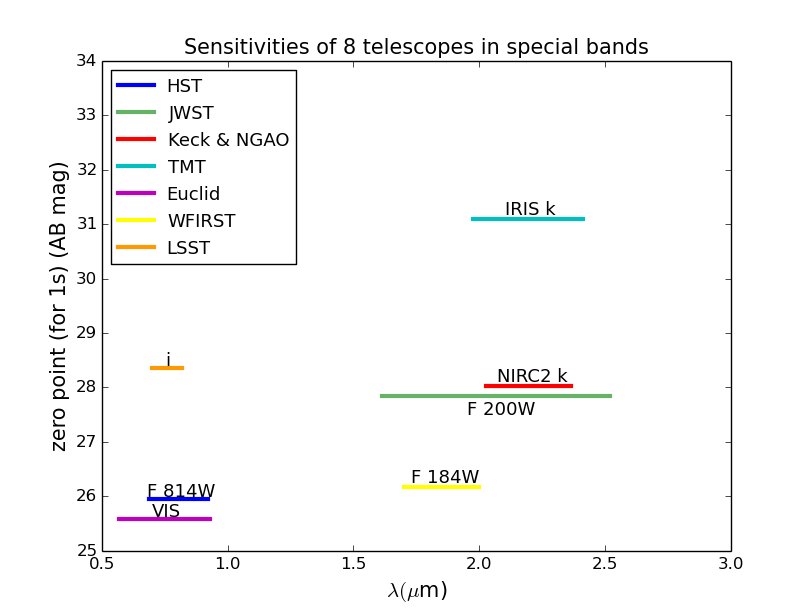
\includegraphics[width=0.9\textwidth]{figures/wavelength_zp.png}
\end{center}
\caption{Zero points in AB magnitudes for HST/ACS (blue), JWST/NIRCAM (green), Keck NIRC2  (assumed for both LGSAO and NGAO; red), TMT/IRIS (cyan), Euclid (magenta), WFIRST (yellow) and LSST (orange), corresponding to one count per second. The colored bars indicate the wavelength range of each instrumental setup considered in this work.}
\label{fig:zp_wavelength}
\end{figure}
% ================================================


% ================================================
\begin{figure}
\begin{center}
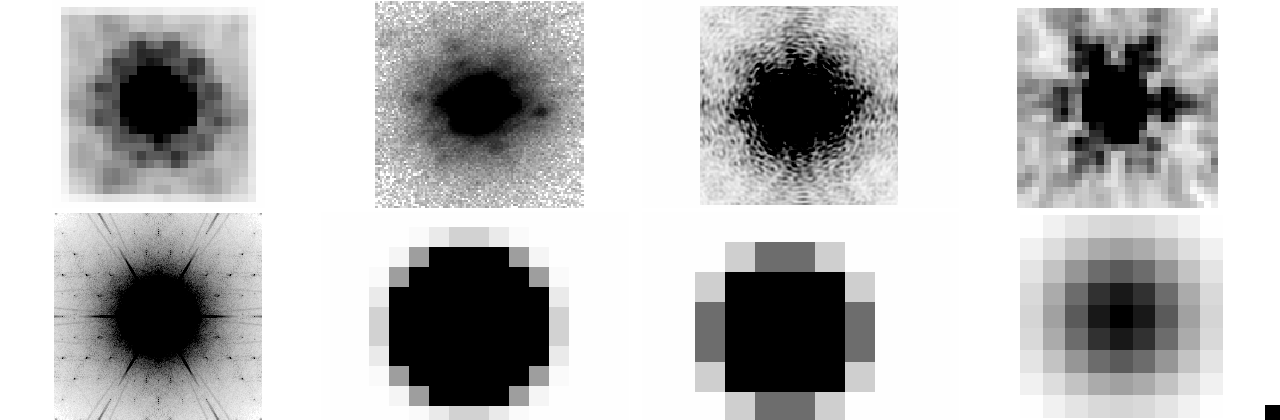
\includegraphics[width=1.0\textwidth]{figures/PSF_montage.png}
\end{center}
\caption{Montage of the point spread functions (PSFs) of each instrument. The upper row, from left to right, represents HST/ACS, Keck/NIRC2+LGSAO, Keck/NIRC2+NGAO, and JWST/NIRCAM. The lower row, from left to right, shows TMT/IRIS, Euclid, WFIRST, and LSST, respectively. Observed or simulated PSFs are used for HST, JWST, Keck (LGSAO \& NGAO), and TMT. Gaussian PSFs are adopted for the other three survey instruments.}
\label{fig:PSF_montage}
\end{figure}
% =================================================



% ================================================
\begin{figure}
\begin{center}
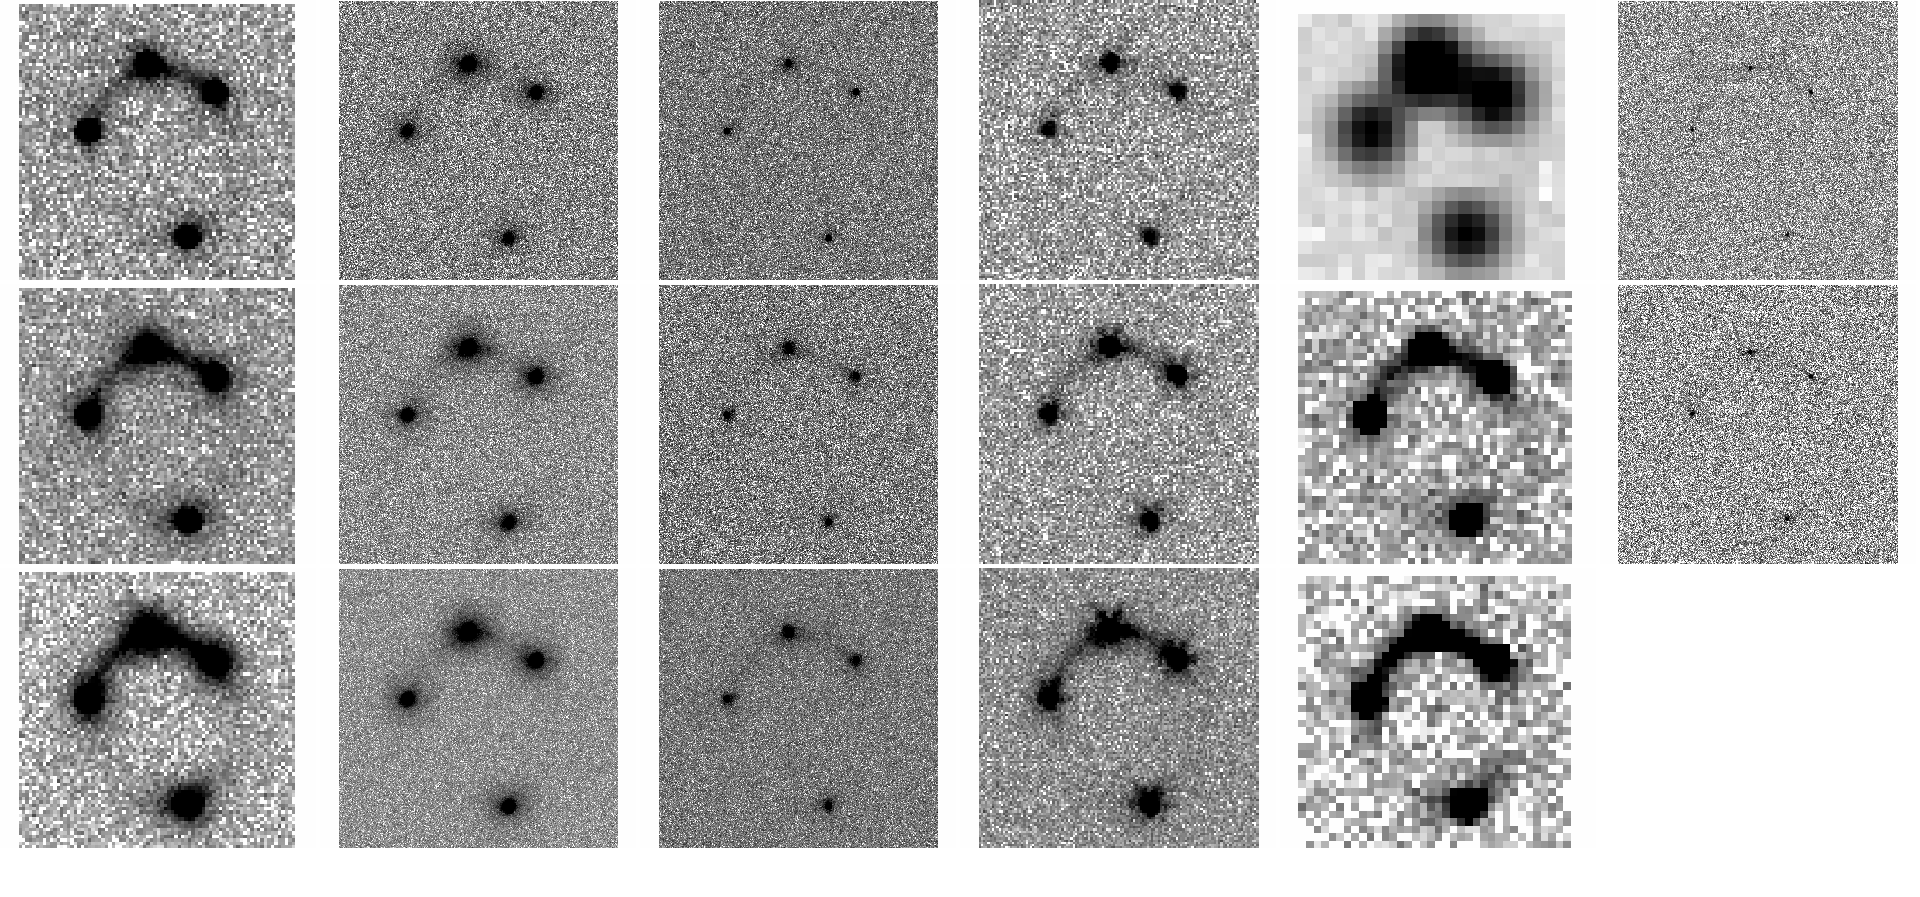
\includegraphics[width=1.0\textwidth]{figures/fainter_system_4QSOimages_all.png}
\end{center}
\caption{Simulations of the fainter lens system with 4 QSO images. The simulated images are all 4$''$ $\times$ 4$''$. The first 4 columns, from left to right, represent HST/ACS, Keck/NIRC2+LGSAO, Keck/NIRC2+NGAO, and JWST/NIRCAM; from top to bottom, the rows correspond to 1/3 $\times$ ``target'' exposure time, ``target'' exposure time, and 3 $\times$ ``target'' exposure time. ``Target'' exposure time is defined as the exposure time that yields 2\% precision on the slope of the mass density profile of the mass model $\gamma'$. The fifth column shows simulations of 3 surveys. From top to bottom we show LSST, Euclid, and WFIRST, with the default survey exposure times (4500s, 2360s, 920s, respectively). The last column shows simulations for TMT with 2 fixed exposure times of 360 seconds and 1080 seconds.}
\label{fig:fainter_4QSOimages_montage}
\end{figure}
% =================================================


% ================================================
\begin{figure}
\begin{center}
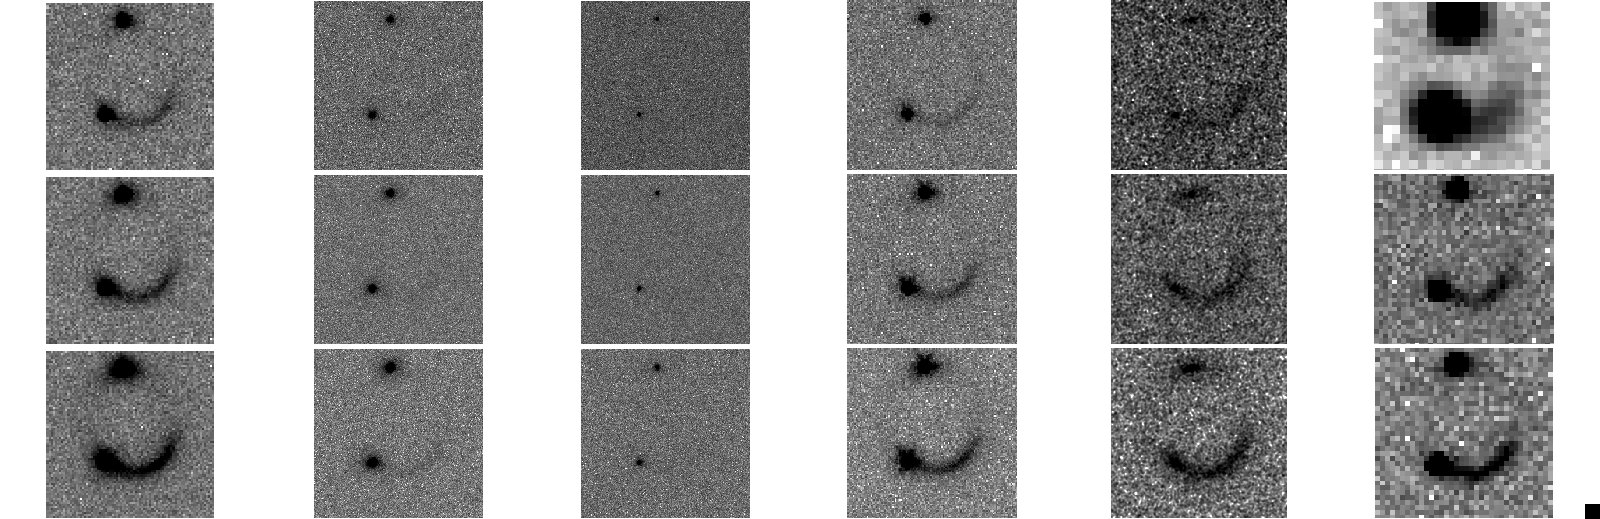
\includegraphics[width=1.0\textwidth]{figures/fainter_system_2QSOimages_all.png}
\end{center}
\caption{Same as Fig. \ref{fig:fainter_4QSOimages_montage}, for the faint double system.}
\label{fig:fainter_2QSOimages_montage}
\end{figure}
% =================================================

% ================================================
\begin{figure}
\begin{center}
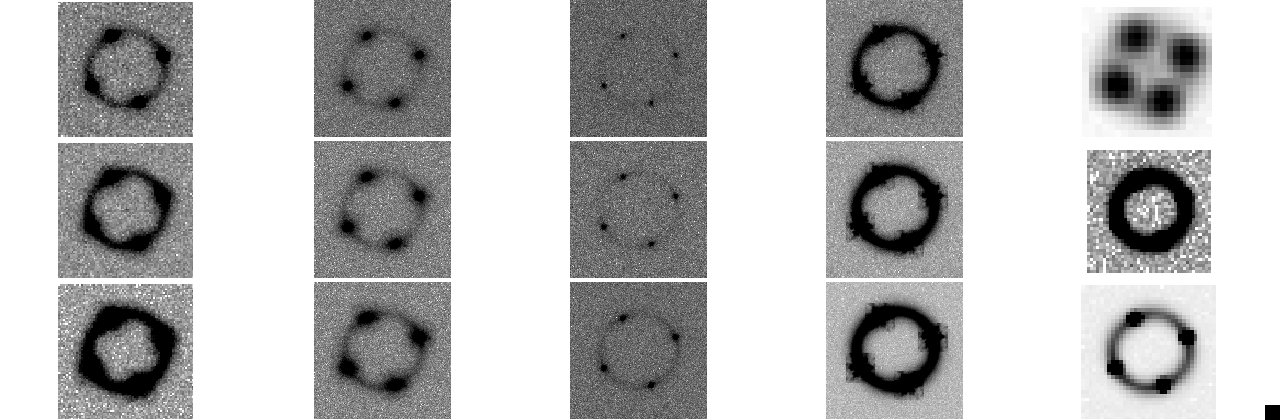
\includegraphics[width=1.0\textwidth]{figures/brighter_system_4QSOimages_all.png}
\end{center}
\caption{Simulations of the bright lens system with 4 QSO images. The simulated images are all 4$''$ $\times$ 4$''$. The first 3 columns, from left to right, represent HST/ACS, Keck/NIRC2+LGSAO, Keck/NIRC2+NGAO; from top to bottom, the rows correspond to 1/3 $\times$ "target" exposure time, "target" exposure time, and 3 $\times$ "target" exposure time. "Target" exposure time is defined as the exposure time that yields 2\% precision on the slope of the mass density profile of the mass model $\gamma'$. The fourth column shows JWST simulations with 3 fixed exposure times: 60, 180, 540 seconds, from top to bottom. The fifth column 
shows simulations of 3 surveys. From top to bottom we show LSST, Euclid, and WFIRST, with the default survey exposure times (4500s, 2360s, 920s, respectively). TMT simulations are not shown since the system is considered too bright to be observed with this telescope in practice. \bf {XLM to remake figure after masking black spot artifacts at the center.}}
\label{fig:brighter_4QSOimages_montage}
\end{figure}
% =================================================


% ================================================
\begin{figure}
\begin{center}
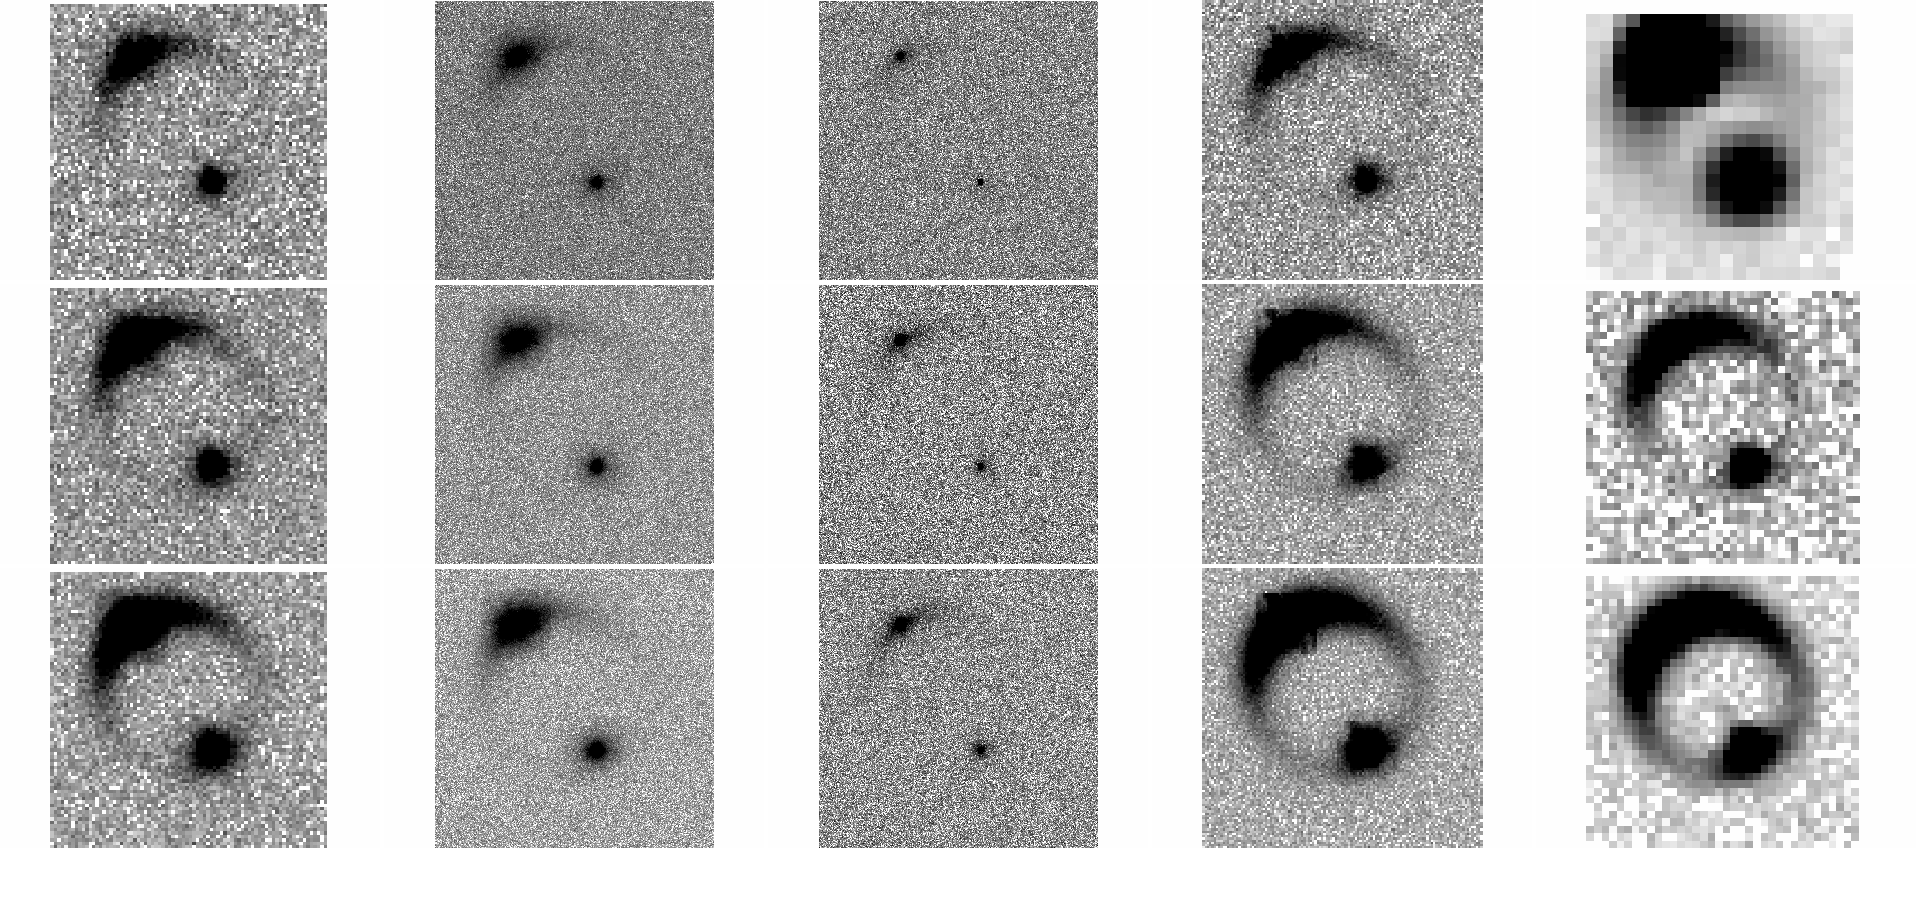
\includegraphics[width=1.0\textwidth]{figures/brighter_system_2QSOimages_all.png}
\end{center}
\caption{Same as Fig. \ref{fig:brighter_4QSOimages_montage}, for the bright double imaged system.}
\label{fig:brighter_2QSOimages_montage}
\end{figure}
% =================================================


% ==================================================
\begin{figure}
\begin{center}
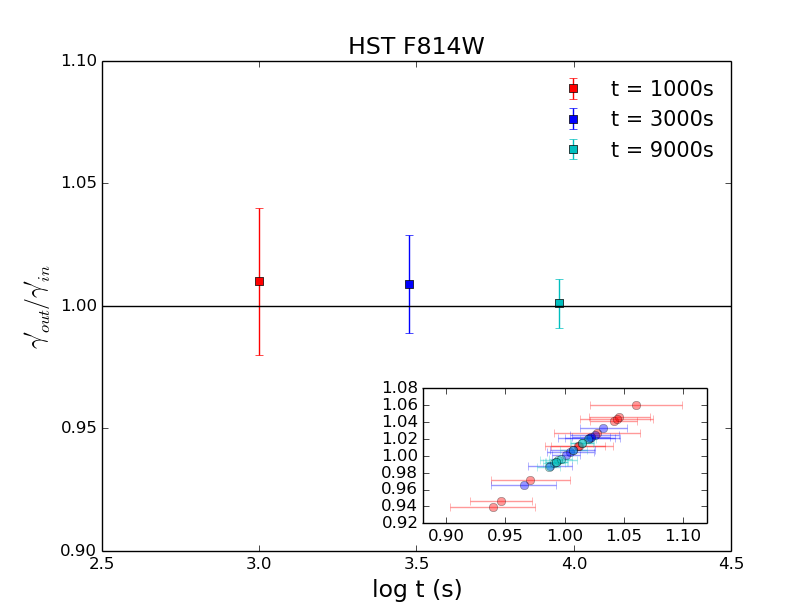
\includegraphics[width=0.48\textwidth]{figures/gamma_135949_4QSOimages_HST.png}
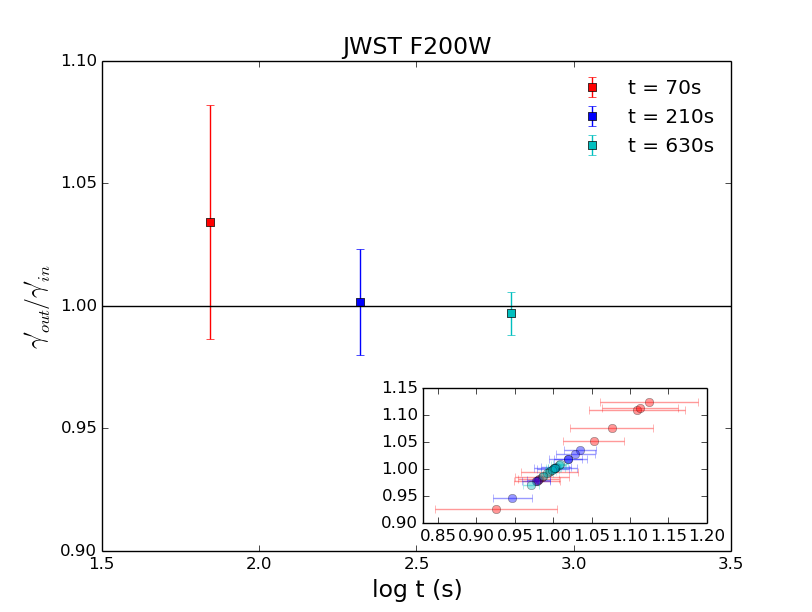
\includegraphics[width=0.48\textwidth]{figures/gamma_135949_4QSOimages_JWST.png} \\
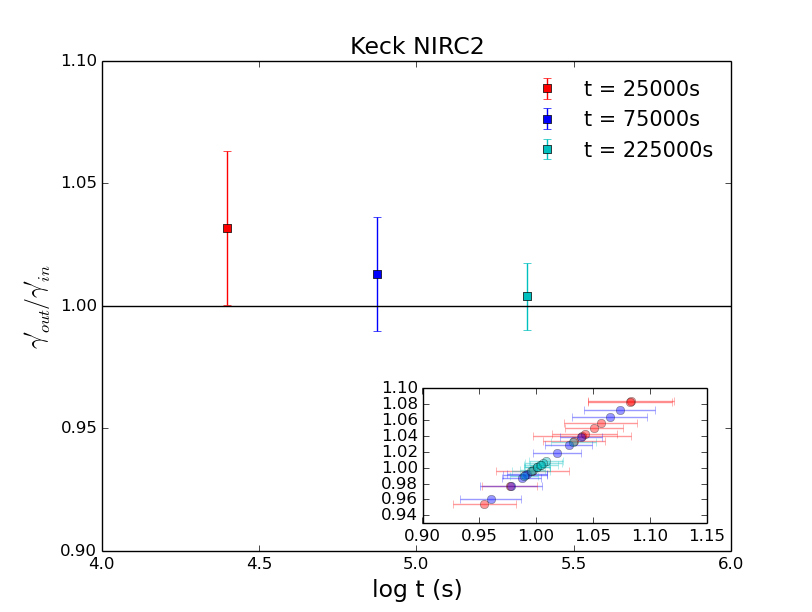
\includegraphics[width=0.48\textwidth]{figures/gamma_135949_4QSOimages_Keck.png}
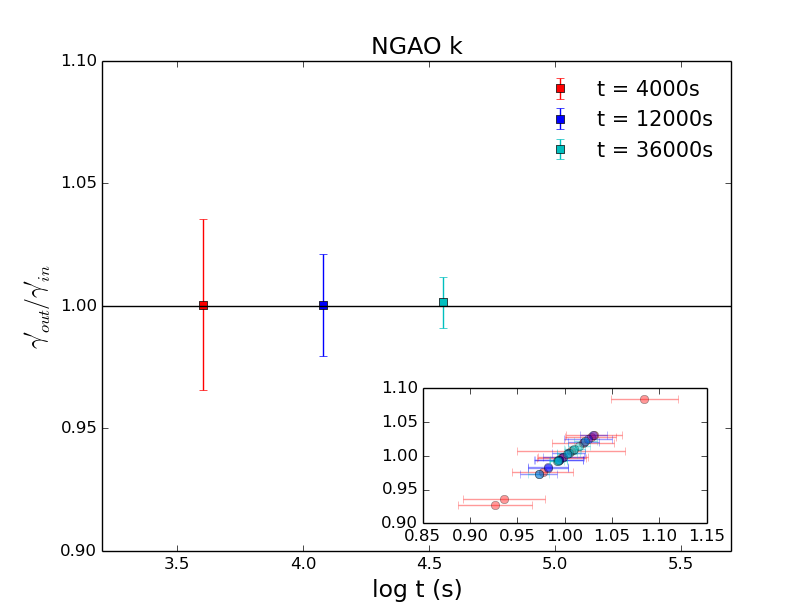
\includegraphics[width=0.48\textwidth]{figures/gamma_135949_4QSOimages_NGAO.png} \\
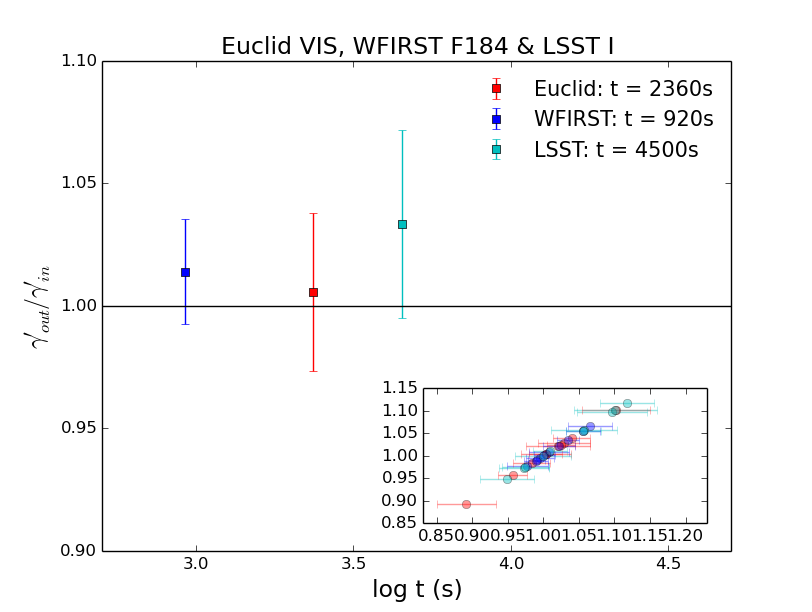
\includegraphics[width=0.48\textwidth]{figures/gamma_135949_4QSOimages_E_W_L.png}
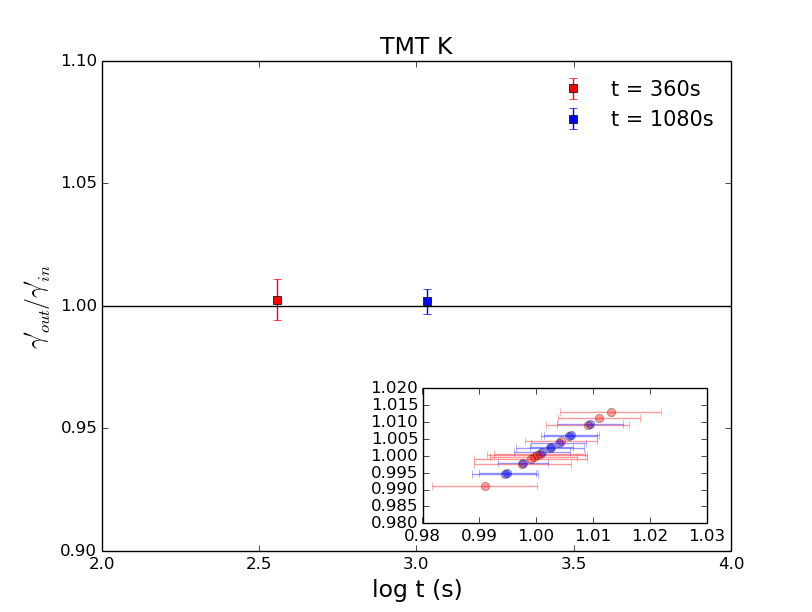
\includegraphics[width=0.48\textwidth]{figures/gamma_135949_4QSOimages_TMT.png}
\end{center}
\caption{Precision on the mass density profile slope $\gamma'$ as a function of exposure time.  This figure shows the results for the fainter lens system with 4 QSO images. The quantity $\gamma'_{in}$ is the input SIE mass slope. The quantity $\gamma'_{out}$ is the output of the inference process.
The insert in each panel shows all 10 simulation results for each exposure time with the same color coding. Note that both axes represent $\gamma'_{out}/\gamma'_{in}$ whereas error bars are only shown on the x-axis for clarity.}
\label{fig:gamma_fainter_4QSOimages}
\end{figure}
% ======================================================


% ==================================================
\begin{figure}
\begin{center}
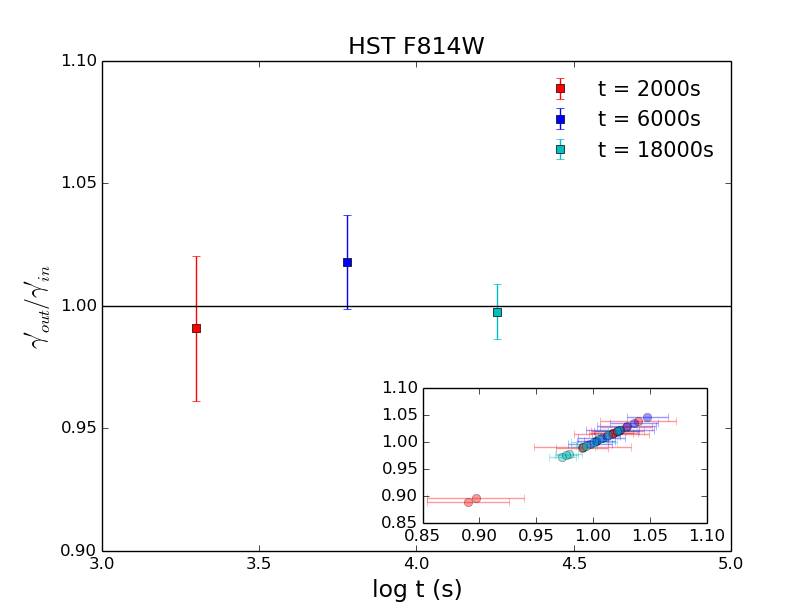
\includegraphics[width=0.48\textwidth]{figures/gamma_135949_anti_2QSOimages_HST.png}
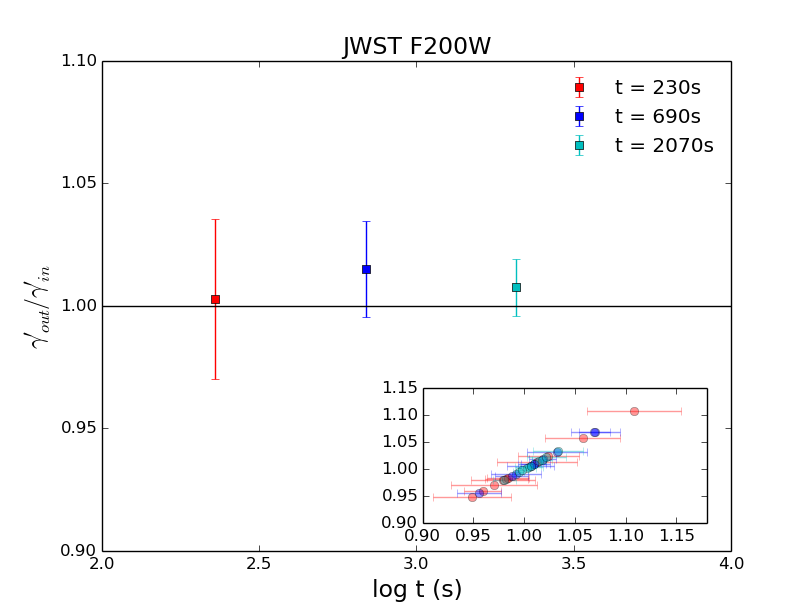
\includegraphics[width=0.48\textwidth]{figures/gamma_135949_anti_2QSOimages_JWST.png} \\
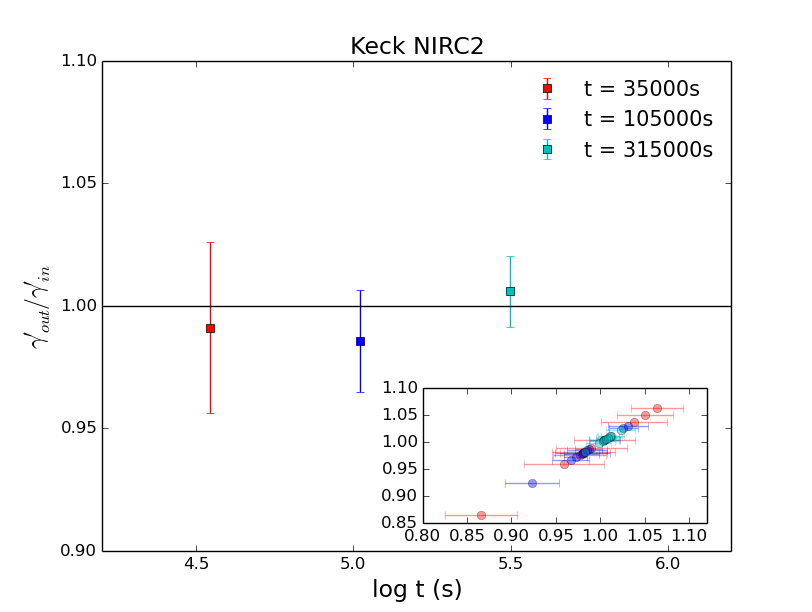
\includegraphics[width=0.48\textwidth]{figures/gamma_135949_anti_2QSOimages_Keck.png}
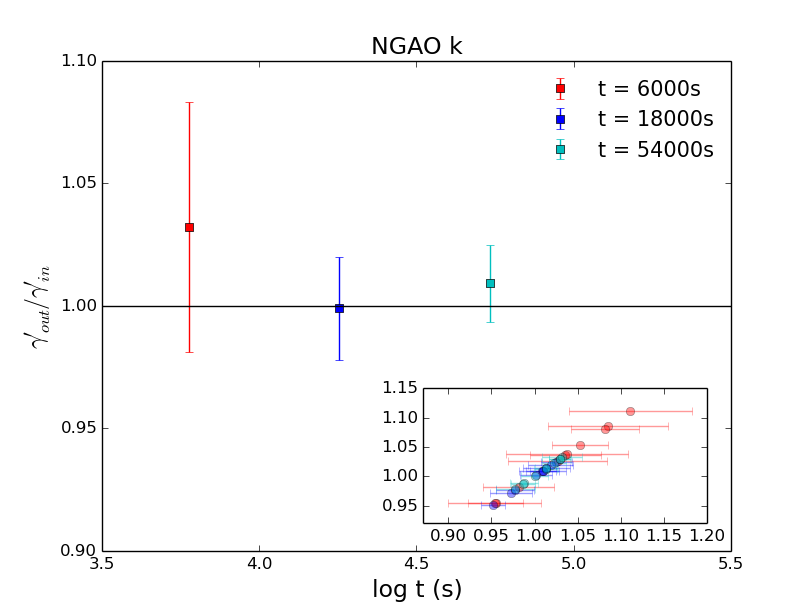
\includegraphics[width=0.48\textwidth]{figures/gamma_135949_anti_2QSOimages_NGAO.png} \\
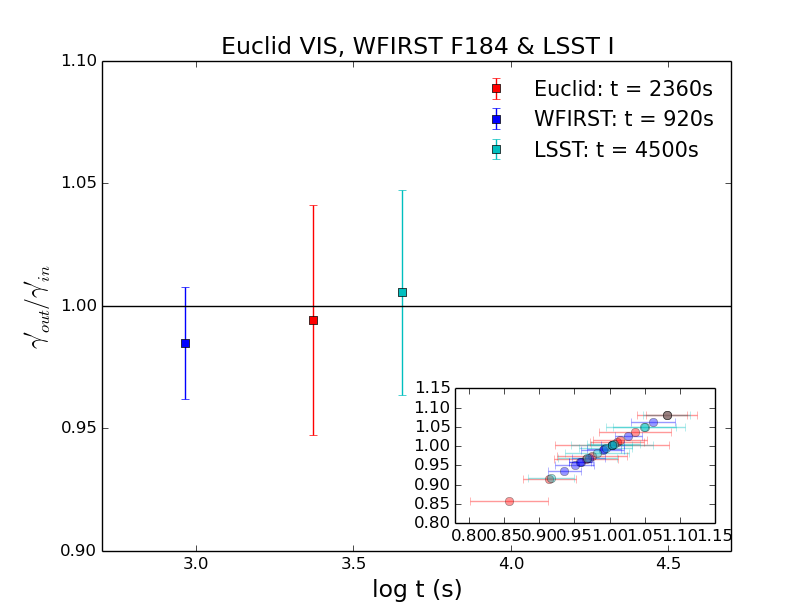
\includegraphics[width=0.48\textwidth]{figures/gamma_135949_anti_2QSOimages_EWL.png}
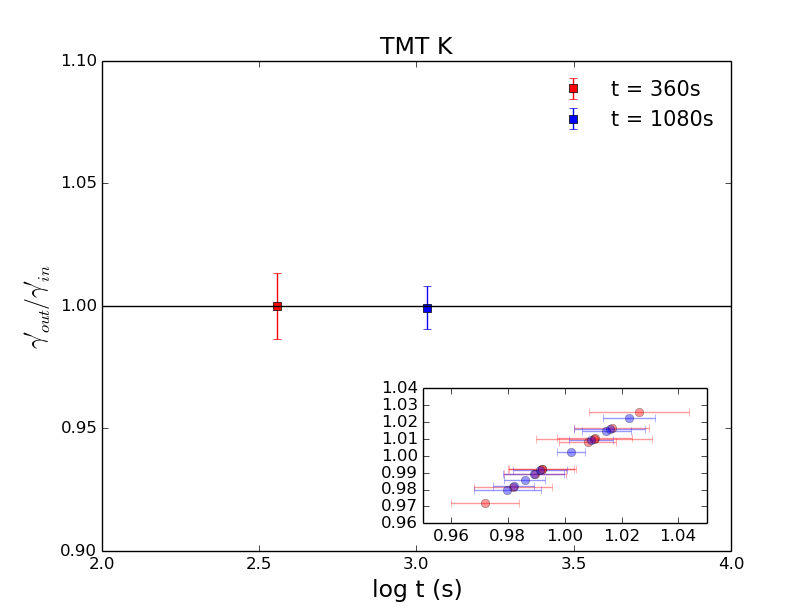
\includegraphics[width=0.48\textwidth]{figures/gamma_135949_anti_2QSOimages_TMT.png}
\end{center}
\caption{Same as Fig.~\ref{fig:gamma_fainter_4QSOimages} for the fainter lens system with 2 images.
\label{fig:gamma_fainter_2QSOimages}}
\end{figure}
% ======================================================

% ==================================================
\begin{figure}
\begin{center}
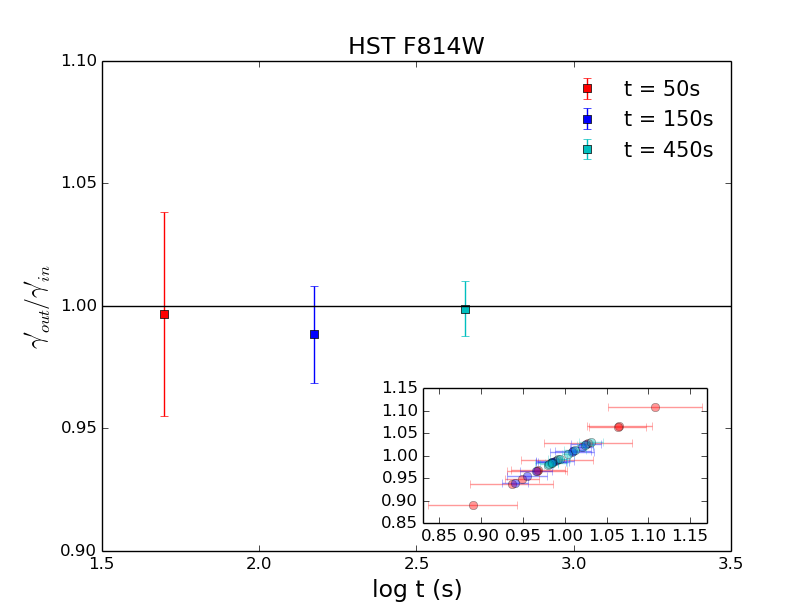
\includegraphics[width=0.48\textwidth]{figures/gamma_0330_anti_4QSOimages_HST.png}
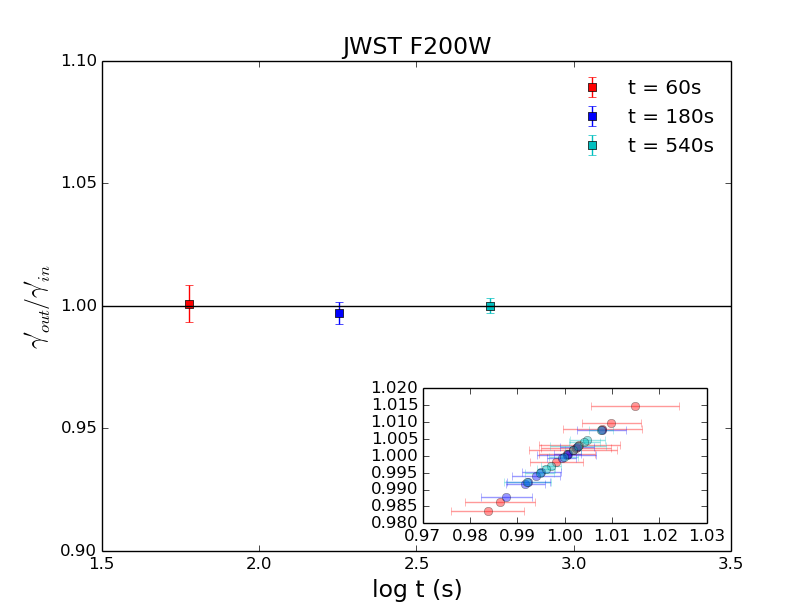
\includegraphics[width=0.48\textwidth]{figures/gamma_0330_anti_4QSOimages_JWST.png} \\
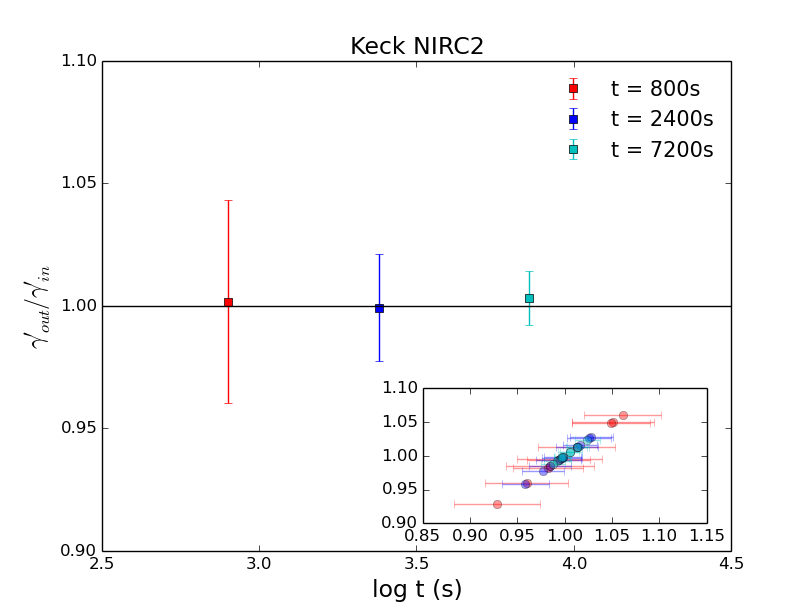
\includegraphics[width=0.48\textwidth]{figures/gamma_0330_anti_4QSOimages_Keck.png}
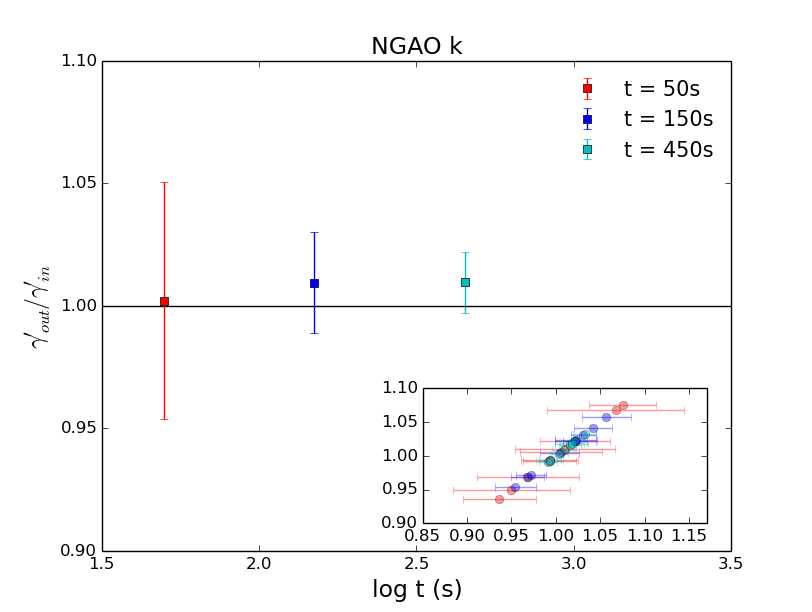
\includegraphics[width=0.48\textwidth]{figures/gamma_0330_anti_4QSOimages_NGAO.png} \\
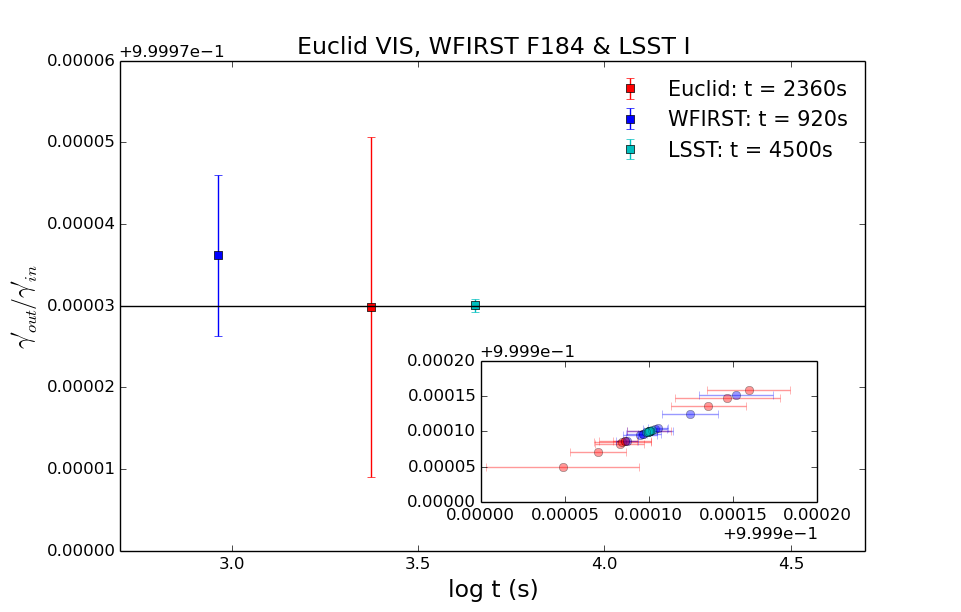
\includegraphics[width=0.48\textwidth]{figures/gamma_0330_anti_4QSOimages_EWL.png}
\end{center}
\caption{Same as Fig.~\ref{fig:gamma_fainter_4QSOimages} for the brighter lens system with 4 images.
\label{fig:gamma_brighter_4QSOimages}}
\end{figure}
% ======================================================

% ==================================================
\begin{figure}
\begin{center}
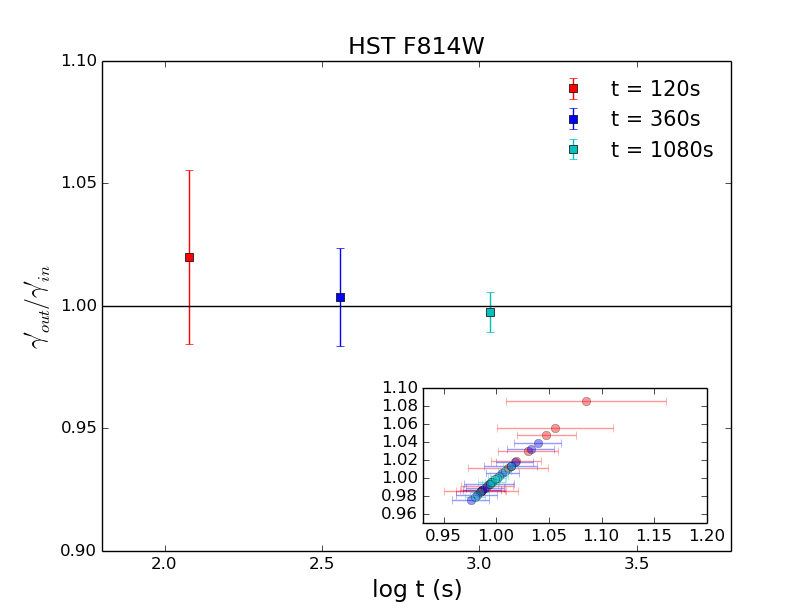
\includegraphics[width=0.48\textwidth]{figures/gamma_0330_2QSOimages_HST.png}
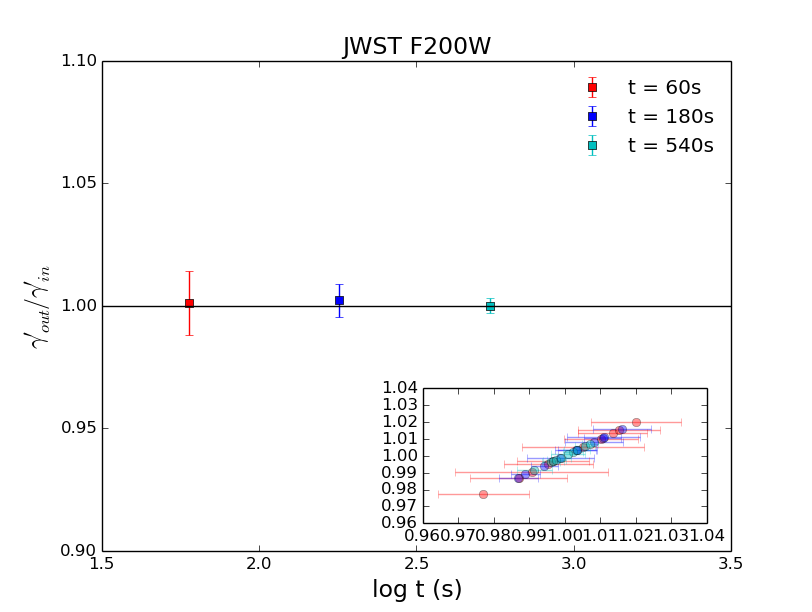
\includegraphics[width=0.48\textwidth]{figures/gamma_0330_2QSOimages_JWST.png} \\
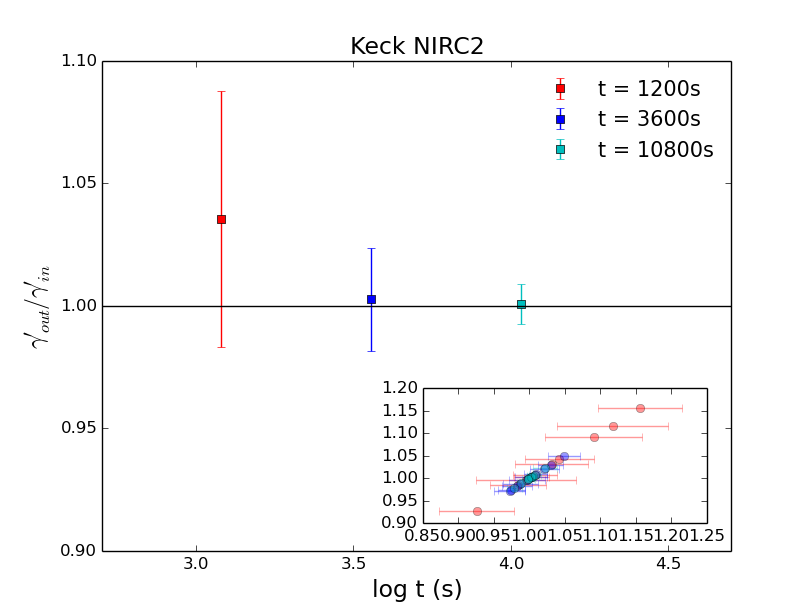
\includegraphics[width=0.48\textwidth]{figures/gamma_0330_2QSOimages_Keck.png}
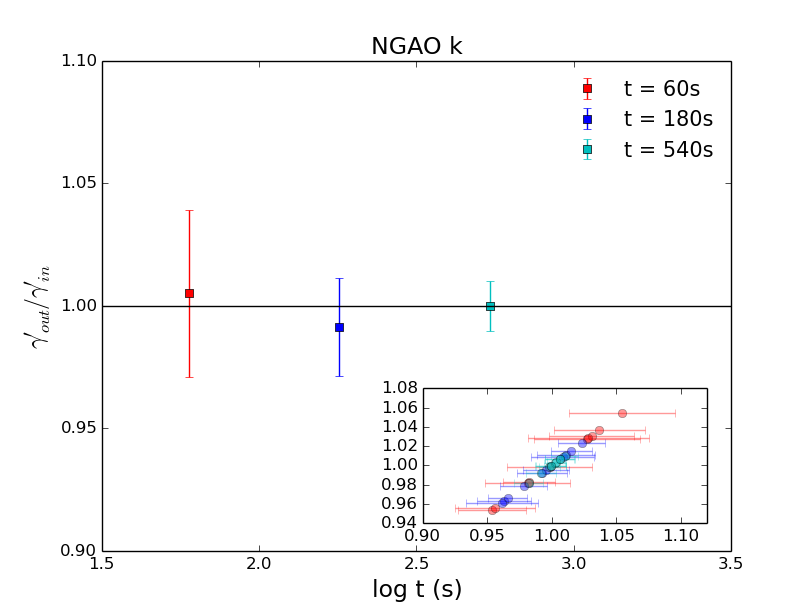
\includegraphics[width=0.48\textwidth]{figures/gamma_0330_2QSOimages_NGAO.png} \\
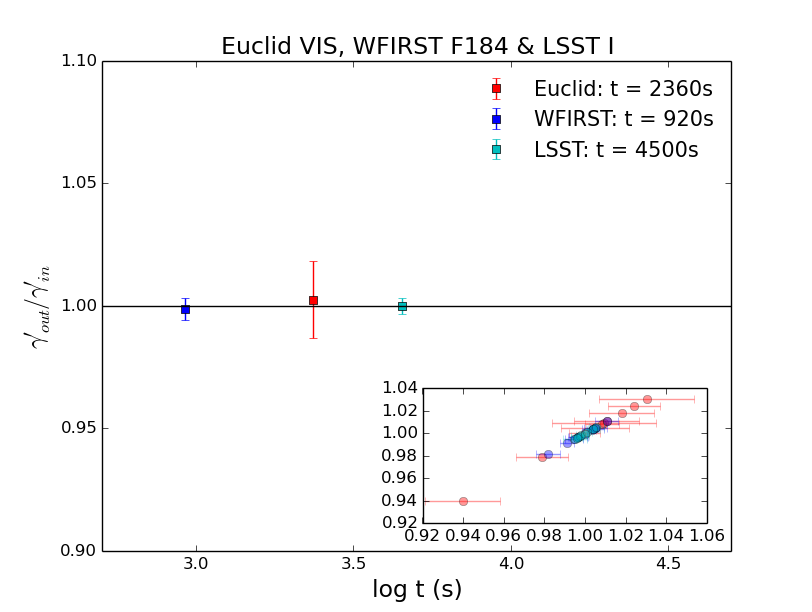
\includegraphics[width=0.48\textwidth]{figures/gamma_0330_2QSOimages_E_W_L.png}
\end{center}
\caption{Same as Fig.~\ref{fig:gamma_fainter_4QSOimages} for the brighter lens system with 2 images.
\label{fig:gamma_brighter_2QSOimages}}
\end{figure}
% ======================================================

\end{document}


\subsection{Selected Realistic Lens Systems}
For wider analysis we plan to We choose a lens from the Sloan Lens ACS
Survey (SLACS; Bolton et al. 2008 \cite{2008ApJ...682..964B}; Auger et
al. 2009 \cite{2009ApJ...705.1099A})
